\documentclass[12pt]{article}
\usepackage{titlesec}
\newcommand{\sectionbreak}{\clearpage}

\usepackage{fontspec}
\usepackage{booktabs}
\usepackage{longtable}
\usepackage{multirow}
\usepackage[autocite=inline,backend=bibtex,sorting=none]{biblatex}
\usepackage{pdfpages}

\addbibresource{test.bib}

\setmainfont{Times New Roman}

\titleformat*{\section}{\LARGE\bfseries}
\titleformat*{\subsection}{\Large\bfseries}
\titleformat*{\subsubsection}{\large\bfseries}

\titleformat{\paragraph}
  {\normalfont\large\bfseries}{\theparagraph}{1em}{}
\titlespacing*{\paragraph}{0pt}{3.25ex plus 1ex minus .2ex}{0ex plus .2ex}

\titleformat{\subparagraph}
  {\normalfont\normalsize\bfseries}{\subparagraph}{1em}{}
\titlespacing*{\subparagraph}{0pt}{3.25ex plus 1ex minus .2ex}{0ex plus .2ex}

\usepackage{geometry}
\geometry{letterpaper, portrait, margin=1in, left=1.5in}

\usepackage{fancyhdr}

\usepackage{graphicx,grffile}

\usepackage[setpagesize=false, % page size defined by xetex
              unicode=false, % unicode breaks when used with xetex
              xetex]{hyperref}

\makeatletter
\def\maxwidth{\ifdim\Gin@nat@width>\linewidth\linewidth\else\Gin@nat@width\fi}
\def\maxheight{\ifdim\Gin@nat@height>\textheight\textheight\else\Gin@nat@height\fi}
\makeatother
% Scale images if necessary, so that they will not overflow the page
% margins by default, and it is still possible to overwrite the defaults
% using explicit options in \includegraphics[width, height, ...]{}
\setkeys{Gin}{width=\maxwidth,height=\maxheight,keepaspectratio}
\setlength{\parindent}{0pt}
\setlength{\parskip}{6pt plus 2pt minus 1pt}
\setlength{\emergencystretch}{3em}  % prevent overfull lines
\providecommand{\tightlist}{%
  \setlength{\itemsep}{0pt}\setlength{\parskip}{0pt}}

\pagestyle{fancy}
\lhead{}
\chead{}
\rhead{}
\lfoot{}
\cfoot{}
\rfoot{\thepage}

\begin{document}
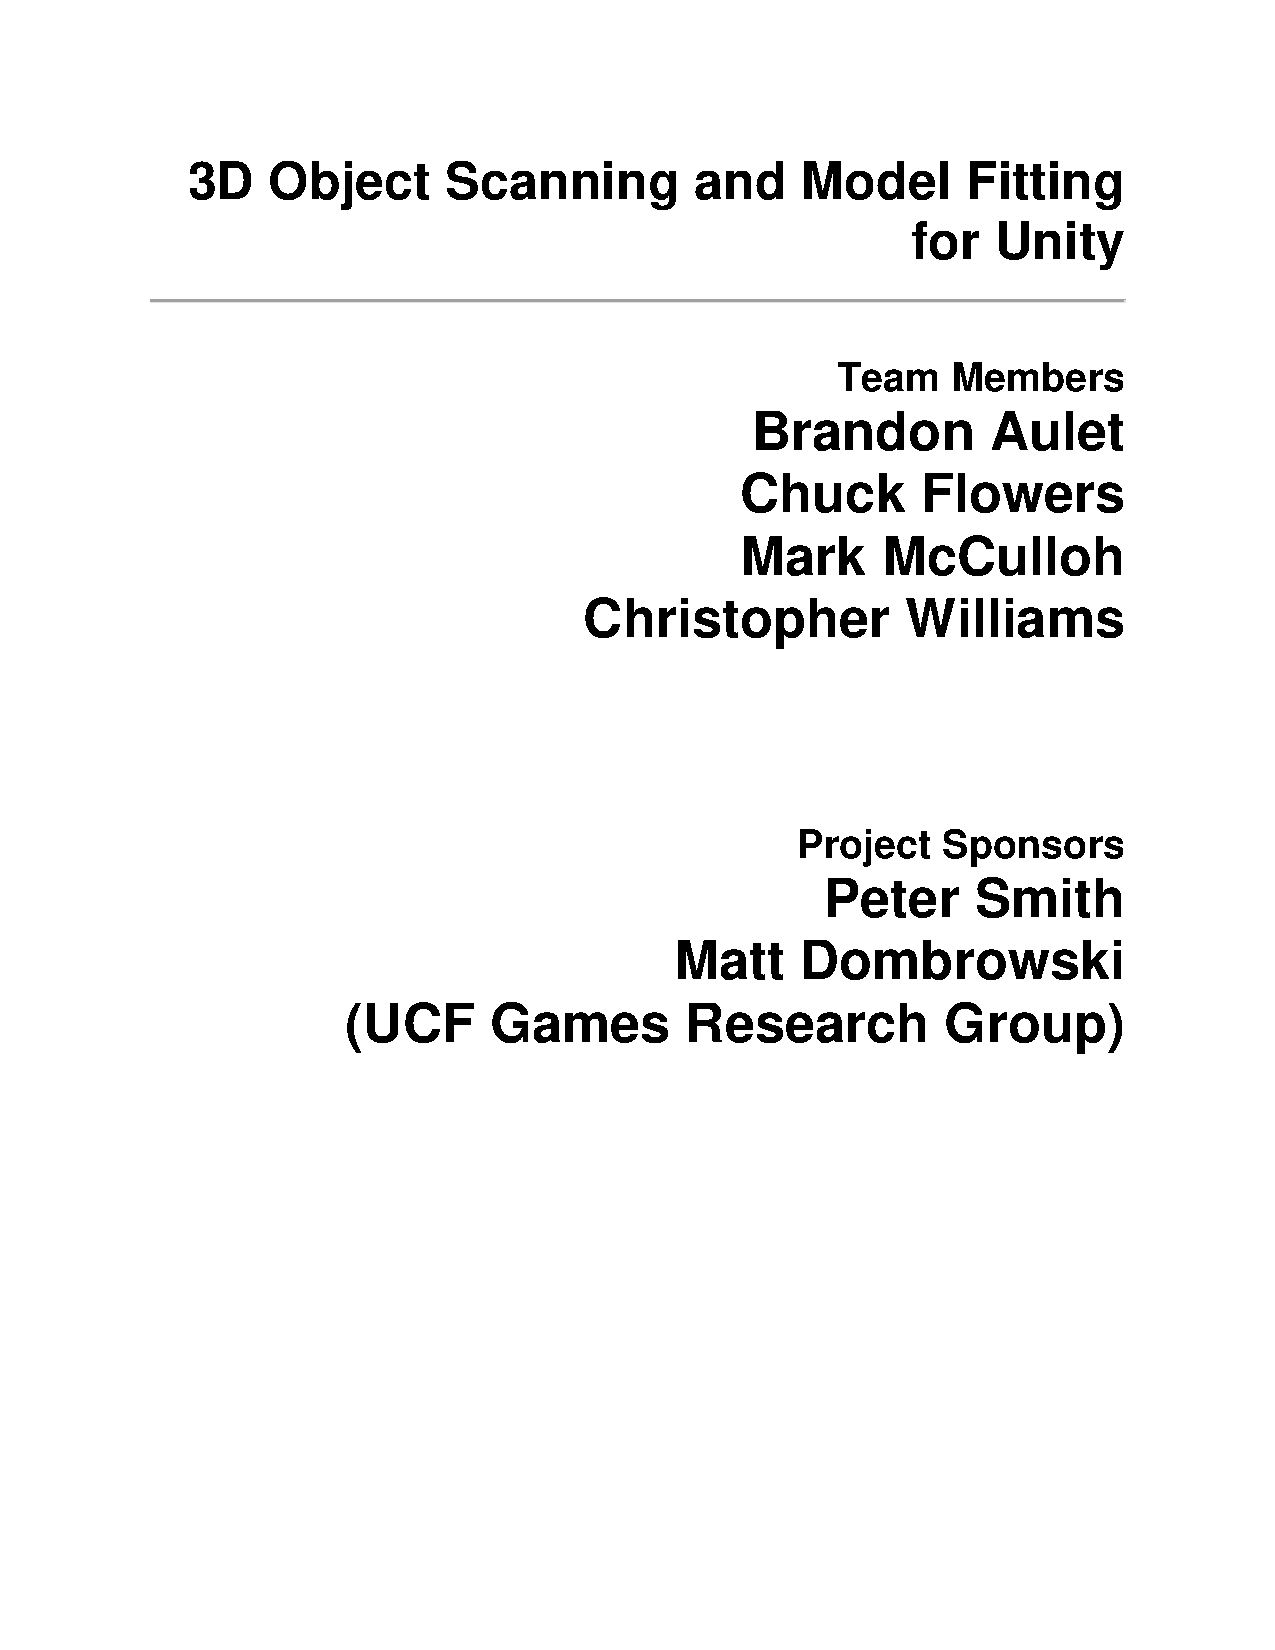
\includepdf[pages=-]{coverPage.pdf}
\pagenumbering{roman} % Start roman numbering
\setcounter{tocdepth}{3}
\tableofcontents

\cleardoublepage
\pagenumbering{arabic} % Switch to normal numbers

\section{Executive Summary}\label{executive-summary}

The purpose of our 3D scanner for Unity is to provide a useful and novel
tool for the Unity game engine. This application will be free to use for
UCF students and potentially added to the Unity Asset Store for use by
indie game developers. The only similar application that is currently
available is Intel® RealSense™, which does not offer the 3D scene
segmentation features to help developers with level creation that we are
planning.

The scanner will consist of three major modules, the first of which
accepts RGB-D images from sensors, like the Microsoft Kinect, and
preprocesses the data to prepare it for the interpreter. The data
interpreter uses this data as input for a computer vision system that
will run a scene understanding algorithm to detect objects and estimate
object poses in 3D space. The last module will take the information
gathered from the computer vision system and transfer this into a format
that can be ported into Unity. Then this module will render the
appropriate models in a Unity scene.

\section{Overview}\label{overview}

\subsection{Broader Impact}\label{broader-impact}

What we are creating is more than just a tool to build prototypes of
videogame levels. It breaks down many of the barriers of entry to
videogame development, softens the learning curve of game design in
general, and makes game design accessible to a wider audience. One of
the barriers to video game design is the time required to build a game.
To build anything of reasonable complexity, a significant investment of
time is required to both design the level and then implement it. Our
tool aims to consolidate the design and implement stages into a single
step. By doing so designs can be quickly evaluated, modified, and
revaluated to arrive at the best course of action in as little time as
possible. This significantly lowers the barriers of entry to small game
studios and single person teams for creating high quality games. This
tool will allow them to develop higher quality games without requiring
the resources that large game studios have. Our tool also softens the
learning curve for learning how to create videogames. The tool
eliminates the need to learn any new skill to design levels. This allows
individuals who are interested in learning about game design to complete
initial projects faster and more quickly evaluate how they feel about
the field of videogame design in general. Finally, our tool makes game
design more accessible to those who would otherwise not be able to
develop videogames via traditional means. By using blocks to design
levels rather than writing code or using a two-dimensional drag and drop
interface, people with underdeveloped computer skills can engage in
videogame design. This means that young children, elderly, and those
lacking finer motor skills would be able to play levels of their own
creation.

\subsection{Personal Motivations}\label{personal-motivations}

\subsubsection{Brandon Aulet}\label{brandon-aulet}

My initial interest in this project stems from my desire to work in the
gaming industry as a software developer. I have been playing videogames
and using computers since I was 4 years old. It has had a huge impact on
my life, and was the main reason for my decision to choose this project.
The further that I have gone in my Computer Science degree, the more
opportunities I try to look for to be able to learn about technology
that the gaming industry uses. This project gives me a great chance to
learn how to manipulate one of the biggest game engines in the market
today.

I was also excited by the prospect of getting to work with hardware and
computer vision algorithms, things that I have not had much experience
with in my time at UCF. This project gives me the opportunity to expand
my knowledge in these fields, making it more interesting and overall
beneficial for my future in and industry by helping me learn to adapt to
different scenarios.

The final reason is that I already had some background in the subject to
begin with. In addition to my Computer Science degree I also pursued a
Digital Media minor, during that time I learned skills that I believed
would help me add to this project such as 3D modeling and a general
proficiency in using Unity from a game designer's perspective. That plus
the connections I made in my Digital Media classes helped me pick this
project as my first choice.

\subsubsection{Timothy Flowers}\label{timothy-flowers}

I first became interested in working on this project because of the
interest I have had in videogames. Although I have never had a very
strong desire to work in the video game industry, I have always enjoyed
videogames as someone who plays them. When I began my course work as a
Computer Science major, I also began to appreciate them on a technical
level. When I saw the pitch for this project I thought it would be a
great opportunity to exercise both my passions in videogames as well and
technical programming.

Apart from my love for videogames, I've also been heavily interested in
graphics. I think the field presents unique programming opportunities
and paradigms that are not often encountered in other areas of computer
science. These opportunities include the usage of highly parallelized
graphics cards as well as the design of shaders which model the behavior
of light when it reflects off different surfaces. I felt like this would
be a good project to further explorer my interest in graphics since
there would be opportunity to process three dimensional models as well
as write an application that interacts with the Unity game engine.

Finally, I found the initial concept of the tool very exciting. When the
implementation is complete, it will allow game designers to eliminate
the need to spend so much time prototyping levels. Our tool should give
them the ability to test an initial concept and then begin to build on
top of it. I get a certain satisfaction at building tools for other
people to use because I feel that in a certain way, I'm responsible for
what people can create with it. To be able to design something that can
help others complete a task much more quickly and efficiently than would
otherwise be possible is what software engineers should always strive to
do.

\subsubsection{Mark McCulloh}\label{mark-mcculloh}

Out of all the possible projects the I could choose for senior design, I
sought after one that provided an interesting outlet for algorithms
related to computer vision whilst also allowing the project to not be
especially daunting due to my lack of experience. I know that I will
fully invest myself in the project if it is interesting and
approachable, regardless of how I feel about my lack of experience. This
project fit that bill immediately, but there were even more positives on
top of that.

I spend a lot of my leisure time both playing and creating games, so it
was natural for me to choose a project that integrates with that culture
and helps others in the same field. The love the idea that I could
create a tool that students of game development can use to develop their
skills or simply have fun visualizing their creativity. I have a hope
that this tool is something that people would actually want to use.

Our project at first seems to lack requirements in a structures way, but
there is a large open field of possibilities that we can tap into. I see
Senior Design as a way to sharpen my skills as a programmer whilst
creating something that I can be proud of, and I consider this project
as a way to accomplish the goals set by my outlook.

\subsubsection{Christopher Williams}\label{christopher-williams}

I had previously suggested a Senior Design project similar to this, but
utilizing procedural generation techniques. I wanted to assist game
developers in level creation by creating procedurally generated
assets/levels as a tool for the Unity or Unreal Engine. This project
gives the same satisfaction in assisting game developers to increase
their efficiency in level prototyping and will allow me to work with the
Unity Game Engine as I intended.

I had not considered that my experience with Computer Vision could help
with game development and I am excited to apply my experience in this
field and learn much more. I am already familiar with resources for
potential previous implementations of Computer Vision systems in 3D
scene processing and reproduction. I enjoy researching the field of
computer vision and hope to write an original implementation for this
project alongside Mark.

I have always been enthralled with the game development process and I am
excited to have a chance to contribute. My career plans are still an
open book at this point in my life and I feel that this project could
even open a door to future game development positions. Consisting of
both computer vision systems and game development methodologies, this
project combines two fields that I am passionate about.

\section{Specifications}\label{specifications}

\subsection{Goals}\label{goals}

Users of Unity will be able to utilize our system turn blocks laid out
on a flat surface into untextured unity models, each of which are
positioned, scaled, and oriented analogous to their real-life
counterparts relative to a current Unity scene. While in Unity, users
may initiate a plugin interface to start capturing their proper camera
and consequently capture images of the real-life block scene. The
untextured objects will appear in the scene when the plugin concludes
its execution.

\subsection{Requirements}\label{requirements}

We have divided up the requirements into two categories: Necessary
Features and Possible Features. Necessary Features contains what is
required for our minimal viable product. Without these, our product is
incomplete. Possible Features contains capabilities we would like for
our product to have but are not mandatory for the final deliverable.

\subsubsection{Necessary Features}\label{necessary-features}

\begin{enumerate}
\def\labelenumi{\arabic{enumi}.}
\tightlist
\item
  The system functions on the Windows platform
\item
  The system is fully invoked enclosed within the Unity platform
\item
  The system takes data from pictures taken from within the system
\item
  The system can interpret a single vertical layer of blocks (minimal
  occlusion) on a flat surface
\item
  The system analyses RGB-D data to calculate objects' placements and
  orientations
\item
  The system uses object data to create and place models into an
  established Unity scene
\end{enumerate}

\subsubsection{Possible Features}\label{possible-features}

\begin{enumerate}
\def\labelenumi{\arabic{enumi}.}
\tightlist
\item
  The system has Linux and OSX compatibility
\item
  The system can take and analyse RGB or RGB-D data
\item
  The system can interpret multiple vertical layers of blocks on a flat
  surface
\item
  The system will have a similar counterpart to work in the Unreal
  Engine.
\end{enumerate}

\section{Research}\label{research}

The following section contains the entirety of the research we have
conducted thus far. It includes our research into all of our camera
options, multiple computer vision algorithms for object recognition, and
our research into industry standard game engine plugin models and
capabilities.

\subsection{Camera Research}\label{camera-research}

The UCF Games Research Group had several devices available to us for no
charge. These included: Intel® RealSense™ F200, Microsoft Hololens, HTC
Vive, and Microsoft Kinect. The following is an analysis as to the
suitability of each of the devices.

\subsubsection{HTC Vive}\label{htc-vive}

The HTC Vive is a virtual reality headset. Although it does have spatial
scanning capabilities, its primary purpose is to immerse the user into
another reality. This does not make it an ideal device for this task
since it requires visual presence at all times to place the blocks on
the scanning surface as well as awareness of the environment to perform
the actual scanning of the blocks. The head-mounted nature of the device
is not as easy to aim as a hand-held device. The cost of the device also
makes it prohibitively expensive which is not congruent with the
accessibility that we desired our tool to provide.

\subsubsection{Microsoft Hololens}\label{microsoft-hololens}

The Microsoft Hololens is an augmented reality headset that projects
images onto the viewing lens to make it appear as if the images are
sharing the same space as the user. Unlike the HTC Vive, Microsoft
Hololens does not remove the user from the environment. This allows the
user to stay visually engaged in the environment and move about safely.
The Hololens also has the added ability of being untethered which allows
for easy movement independent of the location of the device running the
rest of the application. The primary drawbacks to the use of the
Microsoft Hololens are: battery life, cost, and usability. According to
our sponsors while in use the battery only lasts for approximately two
hours and returning the device to full charge requires approximately
five hours. This does not coincide with our desire to create a tool for
rapid prototyping. While the untethered design is desirable, it does not
justify the sacrifice to be made for battery life. The cost of the
device is also prohibitively expensive. It would not be a resource that
could be acquired easily by small game studios or individual developers.
To maintain the accessibility of our tool a more cost effective device
is needed. Finally, we considered the use of a head mounted device
impractical for our project. The benefit of allowing the user to capture
the spatial data hands free is not significant since the user's hands
would have to be cleared from the workspace before capture could begin.
This means that the user cannot perform any actions with their hands
while capturing the data. This makes the hands free capability of any
head mounted headset insignificant for our project.

\subsubsection{Intel® RealSense™ F200}\label{intel-realsense-f200}

The Intel® RealSense™ F200 camera is a small rectangular camera that
could easily be mounted in a variety of settings. The camera provides
the ability the obtain both color streams and depth streams. Its SDK
includes not only the tools to interface with the device itself, but
also prebuilt algorithms for 3D scanning and other computer vision
applications. The only drawback to the device is that it must be
tethered to the computer via USB. This could make it difficult to
capture all the necessary angles for the construction of the Unity
scene.

\paragraph{Possible Implementations}\label{possible-implementations}

There are four choices of implementation for the Camera module of our
application. They are C\# .NET4, C\# Unity, C\# UWP, and C++. The C++
implementation provides a native interface for the camera and the other
three implementations are wrappers around the C++ implementation. The
four different approaches are described and analyzed below.

\subparagraph{C\# .NET4}\label{c-.net4}

This implementation allows for the .NET4 Framework to interface with the
Intel® RealSense™ F200 camera. We would create a DLL file that provides
access to the data that we wish to retrieve from the camera. This
implementation provides the benefit of allowing me to draw on my
previous .NET development experience. The implementation provides the
benefits of a managed language so no extra time would be spent managing
resources. The primary downsides to this approach would be the
complexity associated with calling an external DLL from Unity, and the
performance loss of using a managed language over a native one. The
additional complexity of using an external DLL should be very minor
since there are only a few points of interaction between the Unity game
engine and the external DLL. The performance loss of using a managed
language should not be of a great concern for this application. The
application is not performing real time data analysis so the need for
the extra performance is not great. The module's primary responsibility
is to gather data from the camera and possibly do some light
preprocessing. Neither of these tasks are time critical so the need of a
native implementation is not necessary.

\subparagraph{C\# Unity}\label{c-unity}

This implementation allows the camera module to be written directly into
a Unity Managed Plugin. One of the benefits of implementing the camera
module within the Unity plugin, is the reduction in complexity of the
project. There will not be the need for us to generate an external DLL
for the camera module and will simplify the structure of the project.
Another benefit to this approach is the automatic memory management that
a managed language provides. This reduces the complexity for the
programmer, allows for faster development, and is less likely to
introduce common errors such as memory leaks into the project.

\subparagraph{C\# UWP}\label{c-uwp}

This implementation allows for the Universal Windows Platform to
interface with the Intel® RealSense™ camera. This would involve creating
a UWP app that would interface with the camera and then transfer the
image data to back to Unity as a saved file. The benefit of creating a
UWP application is that the camera module can be run on all variants of
Windows 10. This means that the module could run on phones without any
code changes if necessary. Since there is no benefit to being able to
run the camera application on a phone, the benefits are not useful to
our project.

\subparagraph{C++}\label{c}

This implementation does not use a wrapper and is a pure native
implementation. This gives the advantage of a boost in performance but
also means that we must handle our own memory management. This module of
the project does require a high level of performance. The camera module
is not required to do any real-time data processing and the amount of
processing that is done in this module is relatively light. The
advantages of a native implementation are not as significant here as
they would be in other applications.

\subparagraph{Final Decision}\label{final-decision}

For this module, it makes the most sense to use the C\# Unity
implementation. Since C\# is managed, the code required is simpler and
less prone to errors being introduced by the programmer. The lack of
real-time processing in the camera module also means that the negative
performance impacts associated with managed code are reduced. Finally,
since the code is incorporated directly into the Unity plugin, the need
to call an external DLL is eliminated and will make the deployment and
maintenance of the project simpler.

\paragraph{Intel® RealSense™ SDK
Overview}\label{intel-realsense-sdk-overview}

The Intel® RealSense™ SDK provides access to the camera as well as
access to some computer vision algorithms. Fundamentally the SDK is
needed so that we can receive the data from the camera and then pass it
along to the computer vision module. All the following information is
available from the Intel® RealSense™ SDK \autocite{IntelSDK}.

\subparagraph{SenseManager}\label{sensemanager}

The \texttt{SenseManager} class is the access point for all other
modules within the Intel® RealSense™ SDK. An instance of the
\texttt{SenseManager} class cannot be created with a constructor but
instead is created with a factory pattern using a static method of the
\texttt{SenseManager} class. The primary purpose of the
\texttt{SenseManager} class is to create \texttt{SampleReader} objects,
initiate the data pipeline for processing, and to control execution of
the pipeline. The exact methods required for these functions in the
``Capturing Data'' section below.

\subparagraph{SampleReader}\label{samplereader}

The \texttt{SampleReader} class provides access to a stream of color
samples, depth samples, or both. The sample reader is obtained through a
member function contained within a \texttt{SenseManager} object. The
type of data that the \texttt{SampleReader} provides is determined by
the parameters of a member function call on the \texttt{SampleReader} in
question. The \texttt{SampleReader} provides properties for accessing
the sample that the pipeline generates.

\subparagraph{Scan3D}\label{scan3d}

The \texttt{Scan3D} class provides high level access to the 3D Scanning
algorithms. It acts as an interface to the \texttt{PreviewImage}
property which displays the current captured image, as well as the
\texttt{Reconstruct} method which builds the three dimensional object
from the acquired frames.

\subparagraph{Image}\label{image}

The \texttt{Image} class provides a means to acquire access to the pixel
data of an image as well as the Image's metadata such as height and
width. Its primary elements of interest within the \texttt{Image} class
are the \texttt{AcquireAccess} method, \texttt{ReleaseAccess} method,
and the \texttt{Info} property. The \texttt{AcquireAccess} method gives
the caller a reference to the underlying image data through the use of
an \texttt{ImageData} object reference. Additional parameters of the
\texttt{AcquireAccess} method can also be used to convert the format of
the pixel data received. The \texttt{AcquireAccess} method must be
followed by a \texttt{ReleaseAccess} method call. The
\texttt{ReleaseAccess} method allows other callers to acquire access to
the image's data. The \texttt{Info} property of the \texttt{Image} is
also of importance as it contains the height, width, and format of the
\texttt{Image}.

\subparagraph{ImageData}\label{imagedata}

The \texttt{ImageData} class is comprised of the actual pixel data. It
contains several methods for converting to and from various array types
as well as some Unity specific and .NET specific types. The array types
are general enough that they can be used to convert to another type of
image representation if the need arises.

\subparagraph{Important Enumerations}\label{important-enumerations}

\texttt{FileFormat} is used to specify the file type used by
\texttt{Scan3D} in the \texttt{Reconstruct} method. There are three
supported file types.

\begin{itemize}
\tightlist
\item
  OBJ
\item
  PLY
\item
  STL
\end{itemize}

\texttt{ImageAccess} is used to as an argument to specify the access
permissions when acquiring an \texttt{ImageData} object with
\texttt{AcquireAccess} method.

\begin{itemize}
\tightlist
\item
  ACCESS\_READ
\item
  ACCESS\_WRITE
\item
  ACCESS\_READ\_WRITE
\end{itemize}

\texttt{PixelFormat} is used as an argument to specify the format to be
returned by the \texttt{AcquireAccess} method. Some of the formats are
exclusive to a certain type of data such as color, depth, or infrared.
There are several pixel formats.

\begin{itemize}
\tightlist
\item
  PIXEL\_FORMAT\_YUY2
\item
  PIXEL\_FORMAT\_NV12
\item
  PIXEL\_FORMAT\_RGB32
\item
  PIXEL\_FORMAT\_RGB24
\item
  PIXEL\_FORMAT\_Y8
\item
  PIXEL\_FORMAT\_Y8\_IR\_RELATIVE
\item
  PIXEL\_FORMAT\_Y16
\item
  PIXEL\_FORMAT\_DEPTH
\item
  PIXEL\_FORMAT\_DEPTH\_RAW
\item
  PIXEL\_FORMAT\_DEPTH\_F32
\item
  PIXEL\_FORMAT\_DEPTH\_CONFIDENCE
\end{itemize}

\texttt{StreamType} is used as an argument to specify the type of stream
to a \texttt{SampleReader} receives. Some of the stream types are not
supported by all Intel® RealSense™ cameras.

\begin{itemize}
\tightlist
\item
  STREAM\_TYPE\_ANY
\item
  STREAM\_TYPE\_COLOR
\item
  STREAM\_TYPE\_DEPTH
\item
  STREAM\_TYPE\_IR
\item
  STREAM\_TYPE\_LEFT
\item
  STREAM\_TYPE\_RIGHT
\end{itemize}

\subparagraph{Capturing Color and Depth
Data}\label{capturing-color-and-depth-data}

The basis of computer vision algorithms is the capture and analysis of
depth and color data In order to begin capturing depth and/or color
data, 4 steps have to be executed.

\begin{enumerate}
\def\labelenumi{\arabic{enumi}.}
\tightlist
\item
  Acquire the \texttt{SenseManager} object by calling the static
  \texttt{SenseManager.CreateInstance} method
\item
  Acquire a \texttt{SampleReader} object by calling the static
  \texttt{SampleReader.Activate} method and passing the acquired
  \texttt{SenseManager} as an argument
\item
  Call the \texttt{EnableStream} method on the acquired
  \texttt{SampleReader} and pass it the type of desired stream
\item
  Call the \texttt{Init} method on the \texttt{SenseManager} with no
  arguments
\end{enumerate}

Once these steps have been completed it is possible to acquire data from
the video pipeline. Acquiring data can be achieved in 3 easy steps

\begin{enumerate}
\def\labelenumi{\arabic{enumi}.}
\tightlist
\item
  Call \texttt{AcquireFrame} on the acquired \texttt{SenseManager}
\item
  Retrieve the \texttt{Sample} Property from the acquired
  \texttt{SampleReader}
\item
  Call \texttt{ReleaseFrame} on the acquired \texttt{SenseManager} when
  frame processing is complete
\end{enumerate}

The above three steps may be repeated as many times as desired for each
frame of data to be captured. Upon completion of data capture. The
\texttt{Close} method or \texttt{Dispose} method must be called on the
acquired \texttt{SenseManager}. Use \texttt{Close} if the
\texttt{SenseManager} instance will be used to stream data later.
Otherwise use \texttt{Dispose} to free all resources associated with the
instance.

\subparagraph{3D Scanning}\label{d-scanning}

The Intel® RealSense™ SDK also provides algorithms for scanning 3D
objects into common 3D file formats including: OBJ, STL, and PLY. The
use of these algorithms is made easy through the Intel® RealSense™ SDK
and does not require much more effort than it does to capture raw color
and depth. The process is very similar to process detailed in the
Capturing Color and Depth Data section above. In order to scan objects
the following steps have to be performed.

\begin{enumerate}
\def\labelenumi{\arabic{enumi}.}
\tightlist
\item
  Acquire the \texttt{SenseManager} by calling the static
  \texttt{SenseManager.CreateInstance} method
\item
  Acquire a \texttt{Scan3D} object by calling the static
  \texttt{Scan3D.Activate} method and passing the acquired
  \texttt{SenseManager} as an argument
\item
  Call the \texttt{Init} method on the \texttt{SenseManager} with no
  arguments
\end{enumerate}

This initializes the pipeline for constructing a 3D object. Once the
pipeline has been initialized the data can begin to be captured. Follow
the following steps to capture an image.

\begin{enumerate}
\def\labelenumi{\arabic{enumi}.}
\tightlist
\item
  Call \texttt{AcquireFrame} on the acquired \texttt{SenseManager}
\item
  Capture the result of the \texttt{Scan3D} object's
  \texttt{PreviewImage} method as an \texttt{Image} object
\item
  Call \texttt{ReleaseFrame} on the acquired \texttt{SenseManager} in
  order to capture the next frame
\end{enumerate}

The above three steps may be repeated as many times as desired for each
frame of data to be captured. After all desired frames have been
captured. The \texttt{Reconstruct} method can be called which will save
the object with the specified file format and file location. Upon
completion of data capture and exporting the data to a file, the
\texttt{Close} method or \texttt{Dispose} method must be called on the
acquired \texttt{SenseManager}. Use \texttt{Close} if the
\texttt{SenseManager} instance will be used to stream data later.
Otherwise use \texttt{Dispose} to free all resources associated with the
instance.

\subparagraph{Dispose Method}\label{dispose-method}

Although C\# is a managed language there are some classes in the Intel®
RealSense™ SDK that do not benefit from automatic garbage collection.
These objects include the \texttt{SenseManager} class and the
\texttt{Image} class. In order for the object to be processed by the
garbage collector, the \texttt{Dispose} method must be called. In order
to ensure that the \texttt{Dispose} is called, it is wise to place the
method call inside of a class destructor or to initialize the
\texttt{SenseManager} in a \texttt{using} block.

\subsubsection{Microsoft Kinect}\label{microsoft-kinect}

The Microsoft Kinect is a rectangular sensor that can provide both depth
and color data. Much like the Intel® RealSense™ F200 camera, its SDK
also includes prebuilt computer vision algorithms in addition to the
standard camera interface functionality. It also shares the disadvantage
of needing to be tethered via USB to the main computing device. The
current mode of the Microsoft Kinect sensor has the additional
disadvantage of needing an adapter for use with a laptop. This increases
the cost of the device as well as marginally increasing the complexity
of the set up for the user.

\paragraph{Possible Implementations}\label{possible-implementations-1}

The Microsoft Kinect API provides three different types of APIs. It
provides APIs for the Windows Runtime, .NET Framework, and Native APIs.
All three APIs use similar naming conventions and therefore skills
learned with one API should be able to easily transfer to another. The
advantages, disadvantages, and types of applications that can be written
with these APIs are detailed below.

\subparagraph{Windows Runtime}\label{windows-runtime}

The Windows Runtime APIs allow Windows Store Apps that interface with
the Microsoft Kinect to be written. These APIs can be accessed by any
language that supports the Windows Runtime including C\# and Visual
Basic. The APIs are managed which allow for automatic garbage collection
and memory allocation. Since Windows Store apps have to be distributed
through the Windows Store, we are not interested in this implementation.
We want to be able to package and distribute our plugin together so
having to download one component from the store and another component
from another location is not ideal. We would also have to communicate
the data captured by the Microsoft Kinect to the game engine using a
localhost loopback or saved file.

\subparagraph{.NET Framework}\label{net-framework}

The .NET Framework APIs allow WPF applications to interface with the
Microsoft Kinect. WPF applications are also managed so they carry the
same garbage collection and memory allocation benefits as mentioned in
the Windows Runtime APIs. WPF also supports both C\# and Visual Basic.
Unlike Windows Runtime applications, WPF applications can be distributed
easily outside of a storefront. We would still likely have to use the
same method to transfer data to the game engine.

\subparagraph{Native APIs}\label{native-apis}

The Native APIs differ from the previous two implementations in that
they do not include garbage collection or memory allocation. Both of
these functions have to be explicitly handled by the programmer using
the APIs. This can slow down implementation since extra code has to be
written. It would also require additional diligence during testing to
ensure that there are no memory leaks. The benefit to using the native
implementation is additional performance but the majority of our
computation time is likely to be invested in the computer vision
algorithms and processing and not the data capture itself.

\paragraph{Microsoft Kinect SDK
Overview}\label{microsoft-kinect-sdk-overview}

The following is a brief description of classes from the SDK as they
would be useful to our project. All the information is available in the
Microsoft Kinect SDK Documentation in Appendix B.

\subparagraph{KinectSensor}\label{kinectsensor}

The \texttt{KinectSensor} class is used as the primary interface to the
Microsoft Kinect. The \texttt{KinectSensor} adopts a singleton pattern
by using a static method to return an instance of the
\texttt{KinectSensor} class. Once an instance has been obtained all
other access to the sensor is handled through the instance.

\subparagraph{DepthFrameSource}\label{depthframesource}

The \texttt{DepthFrameSource} class gives access to
\texttt{DepthFrameReader} objects through a simple \texttt{OpenReader}
method. Also includes properties representing the reliable distances
that the Microsoft Kinect can read data.

\subparagraph{DepthFrameReader}\label{depthframereader}

The \texttt{DepthFrameReader} class is used to capture
\texttt{DepthFrame} objects which represent actual data. The frames can
be captured by subscribing an event handler to the \texttt{FrameArrived}
member event or by making a call to the \texttt{AcquireLatestFrame}
method.

\subparagraph{DepthFrame}\label{depthframe}

The \texttt{DepthFrame} class represents a single moment of depth data
capture. The data is represented as an image where the pixels represent
the distance of the given pixel area from the camera. It provides
methods for accessing the underlying pixel data in both buffer and array
forms.

\subparagraph{ColorFrameSource}\label{colorframesource}

The \texttt{ColorFrameSource} class gives access to
\texttt{ColorFrameReader} objects through a simple \texttt{OpenReader}
method. Also includes properties representing the reliable distances
that the Microsoft Kinect can read data.

\subparagraph{ColorFrameReader}\label{colorframereader}

The \texttt{ColorFrameReader} class is used to capture
\texttt{ColorFrame} objects which represent actual data. The frames can
be captured by subscribing an event handler to the \texttt{FrameArrived}
member event or by making a call to the \texttt{AcquireLatestFrame}
method.

\subparagraph{ColorFrame}\label{colorframe}

The \texttt{ColorFrame} class represents a single moment of color data
capture. The data is represented as an image where the pixels represent
the color of the given pixel area as recorded by the camera. It provides
methods for accessing the underlying pixel data as either a buffer or an
array.

\subparagraph{Capturing Color and Depth
Data}\label{capturing-color-and-depth-data-1}

The following steps should be followed in order to initialize the
Microsoft Kinect camera sensor for data collection.

\begin{enumerate}
\def\labelenumi{\arabic{enumi}.}
\tightlist
\item
  Acquire an instance of the \texttt{KinectSensor} class by calling
  \texttt{KinectSensor.GetDefault()}
\item
  Call the \texttt{Open()} member method on the acquired
  \texttt{KinectSensor} object
\item
  Call the \texttt{OpenReader()} member method on the acquired
  \texttt{KinectSensor} object's \texttt{ColorFrameSource} property to
  acquire a \texttt{ColorFrameReader}
\item
  Call the \texttt{OpenReader()} member method on the acquired
  \texttt{KinectSensor} object's \texttt{DepthFrameSource} property to
  acquire a \texttt{DepthFrameReader}
\end{enumerate}

Once the previous steps have been completed the data can begin to be
captured from the sensor. Perform the following steps in order to
acquire color and depth data.

\begin{enumerate}
\def\labelenumi{\arabic{enumi}.}
\tightlist
\item
  Call the \texttt{AcquireLatestFrame} method on the acquired
  \texttt{ColorFrameReader} to obtain a \texttt{ColorFrame}
\item
  Call the \texttt{AcquireLatestFrame} method on the acquired
  \texttt{DepthFrameReader} to obtain a \texttt{DepthFrame}
\end{enumerate}

Once the previous steps have been performed the data can be read from
the two acquired frames. Once the processing is complete be sure to call
the \texttt{Close()} member method on the two acquired frames to release
the system resources. Repeat the previous step as many times as desired.
If no more data needs to be collected, then call the \texttt{Close()}
member method on both the acquired \texttt{ColorFrameReader} and the
acquired \texttt{DepthFrameReader} as well as the acquired
\texttt{KinectSensor} instance.

\subsubsection{Final Decision}\label{final-decision-1}

In addition to all of the advantages and disadvantages of each camera
device described above, it is also important to the compare the system
requirements. Our project team has the computing power to use each of
these devices and we feel it is also reasonable to assume that game
developers would also already have devices of this caliber in order to
run high performance games. Even so all the devices compared have
comparable hardware requirements to one another and are noted below
\autocites{ViveRequirements}{KinectRequirements}{IntelRequirements}.

\begin{longtable}[]{@{}llllll@{}}
\toprule
\begin{minipage}[b]{0.14\columnwidth}\raggedright\strut
Sensor\strut
\end{minipage} & \begin{minipage}[b]{0.18\columnwidth}\raggedright\strut
OS\strut
\end{minipage} & \begin{minipage}[b]{0.20\columnwidth}\raggedright\strut
CPU\strut
\end{minipage} & \begin{minipage}[b]{0.10\columnwidth}\raggedright\strut
Memory\strut
\end{minipage} & \begin{minipage}[b]{0.10\columnwidth}\raggedright\strut
I/O\strut
\end{minipage} & \begin{minipage}[b]{0.11\columnwidth}\raggedright\strut
Misc\strut
\end{minipage}\tabularnewline
\midrule
\endhead
\begin{minipage}[t]{0.14\columnwidth}\raggedright\strut
HTC Vive\strut
\end{minipage} & \begin{minipage}[t]{0.18\columnwidth}\raggedright\strut
Win 7 SP1; Win 8.1; Win 10\strut
\end{minipage} & \begin{minipage}[t]{0.20\columnwidth}\raggedright\strut
Intel® Core™ i5-4590 \textless{}\strut
\end{minipage} & \begin{minipage}[t]{0.10\columnwidth}\raggedright\strut
4GB \textless{}\strut
\end{minipage} & \begin{minipage}[t]{0.10\columnwidth}\raggedright\strut
USB 2.0\strut
\end{minipage} & \begin{minipage}[t]{0.11\columnwidth}\raggedright\strut
Unspecified\strut
\end{minipage}\tabularnewline
\begin{minipage}[t]{0.14\columnwidth}\raggedright\strut
Microsoft Hololens\strut
\end{minipage} & \begin{minipage}[t]{0.18\columnwidth}\raggedright\strut
N/A (Untethered)\strut
\end{minipage} & \begin{minipage}[t]{0.20\columnwidth}\raggedright\strut
N/A (Untethered)\strut
\end{minipage} & \begin{minipage}[t]{0.10\columnwidth}\raggedright\strut
N/A (Untethered)\strut
\end{minipage} & \begin{minipage}[t]{0.10\columnwidth}\raggedright\strut
N/A (Untethered)\strut
\end{minipage} & \begin{minipage}[t]{0.11\columnwidth}\raggedright\strut
N/A (Untethered)\strut
\end{minipage}\tabularnewline
\begin{minipage}[t]{0.14\columnwidth}\raggedright\strut
Intel® RealSense™ F200\strut
\end{minipage} & \begin{minipage}[t]{0.18\columnwidth}\raggedright\strut
Win 8.1(x86/x64); Win 10 (x64)\strut
\end{minipage} & \begin{minipage}[t]{0.20\columnwidth}\raggedright\strut
4th or 5th Generation Intel® Core™\strut
\end{minipage} & \begin{minipage}[t]{0.10\columnwidth}\raggedright\strut
Unspecified\strut
\end{minipage} & \begin{minipage}[t]{0.10\columnwidth}\raggedright\strut
USB\strut
\end{minipage} & \begin{minipage}[t]{0.11\columnwidth}\raggedright\strut
Unspecified\strut
\end{minipage}\tabularnewline
\begin{minipage}[t]{0.14\columnwidth}\raggedright\strut
Microsoft Kinect\strut
\end{minipage} & \begin{minipage}[t]{0.18\columnwidth}\raggedright\strut
Win 8 (x64) \textless{}\strut
\end{minipage} & \begin{minipage}[t]{0.20\columnwidth}\raggedright\strut
i7 3.1 GHz (or higher)\strut
\end{minipage} & \begin{minipage}[t]{0.10\columnwidth}\raggedright\strut
4 GB (or higher)\strut
\end{minipage} & \begin{minipage}[t]{0.10\columnwidth}\raggedright\strut
USB 3.0\strut
\end{minipage} & \begin{minipage}[t]{0.11\columnwidth}\raggedright\strut
DirectX 11\strut
\end{minipage}\tabularnewline
\bottomrule
\end{longtable}

We took the HTC Vive and the Microsoft Hololens out of consideration
because we did not feel that a head-mounted device fit with the way
users would interact with our application. Our main decision was
choosing between the Intel® RealSense™ F200 camera and the Microsoft
Kinect. Both sensors had many of the same advantages and disadvantages.
The differentiating factors between the two was the size of the sensor,
cost of the sensor, and the usability of the APIs. It was in these areas
that the aspects of the devices differed enough for us to make our
decision.

The Intel® RealSense™ F200 Camera was marginally cheaper, costing
approximately \$100. This reduced price helps to achieve a greater level
of accessibility for our tool which is an overall goal of our project.
By reducing the costs allows for smaller development teams to expedite
their design workflow. The Intel® RealSense™ F200 also did not require
the additional purchase of an adapter for the sensor which simplifies
the integration for the end user of our tool.

The handheld usability means that camera can be aimed easily and moved
around the workspace as needed. Although the USB tethering of the device
could make certain angles difficult, the use of a rotating platform or a
primary computing device which can be easily moved, could be used to
minimize this difficulty. The use of such solutions would allow images
to be captured from every angle which is necessary for the computer
vision algorithms that we will implement to process the data.

Finally, although the APIs were similar we felt that the documentation
and overall pattern of use found in the Intel® RealSense™ SDK were much
more straightforward and easier to understand. There were also several
simple code examples to help get programmers who were unfamiliar with
the API.

Both the Microsoft Kinect and the Intel® RealSense™ F200 are comparable
devices and in the unlikely event that the Intel® RealSense™ F200 will
not satisfy our requirements, the Microsoft Kinect is a sound
alternative.

\subsection{Computer Vision Research}\label{computer-vision-research}

\subsubsection{Inputs}\label{inputs}

There are two basic input formats for the incoming camera data: Point
Cloud Data (PCD) or RGB-D image pairs. Point Cloud Data provides
millions of data points which provides an implicit high accuracy level.
The difficulty with Point Cloud Data is that minimization or
simplification would be required before processing if we wish to achieve
fast runtimes.

RGB-D image pairs would contain an RGB image alongside a depth image per
frame. This provides a faster runtime more similar to image processing
tasks, but it still provides depth information to make sufficiently
accurate processing results for our purposes. For these reasons we have
chosen to utilize the ability of the Intel® RealSense™ F200 camera to
capture RGB-D image pairs for our application.

The amount of images passed to the computer vision interface is a
crucial detail and will take testing to determine the optimal amount of
images, angles of view, and capture rate.

\subsubsection{Outputs}\label{outputs}

Output from the computer vision interface will mimic the researched
methods in the following section. These algorithms output pose
information usually in the form of metadata. The metadata for our
project will include an estimated object center point in 3D coordinates
based on the camera's viewpoint, which is used to estimate a translation
matrix. That translation matrix, an object rotation matrix, the object's
scale, and a enumerated object type that corresponds with an object
model will be outputted to provide sufficient information to add an
object to a Unity scene. We plan on importing this data directly into
the Unity Game Engine through our plugin interface.

\subsubsection{Training Hardware}\label{training-hardware}

Due to the demand required in the training process, our team will be
using the strongest computer we have available to us. To train our
detection algorithm, we will use Mark's personal laptop, which has the
specifications listed below.

\begin{longtable}[]{@{}cl@{}}
\toprule
\begin{minipage}[b]{0.21\columnwidth}\centering\strut
Component\strut
\end{minipage} & \begin{minipage}[b]{0.35\columnwidth}\raggedright\strut
Specification\strut
\end{minipage}\tabularnewline
\midrule
\endhead
\begin{minipage}[t]{0.21\columnwidth}\centering\strut
CPU\strut
\end{minipage} & \begin{minipage}[t]{0.35\columnwidth}\raggedright\strut
Intel® 6th Generation Core i7\strut
\end{minipage}\tabularnewline
\begin{minipage}[t]{0.21\columnwidth}\centering\strut
OS\strut
\end{minipage} & \begin{minipage}[t]{0.35\columnwidth}\raggedright\strut
Windows 10 Pro\strut
\end{minipage}\tabularnewline
\begin{minipage}[t]{0.21\columnwidth}\centering\strut
Display\strut
\end{minipage} & \begin{minipage}[t]{0.35\columnwidth}\raggedright\strut
15.6" FHD (1920x1080), IPS-Level\strut
\end{minipage}\tabularnewline
\begin{minipage}[t]{0.21\columnwidth}\centering\strut
Chipset\strut
\end{minipage} & \begin{minipage}[t]{0.35\columnwidth}\raggedright\strut
Intel® HM170\strut
\end{minipage}\tabularnewline
\begin{minipage}[t]{0.21\columnwidth}\centering\strut
Graphics\strut
\end{minipage} & \begin{minipage}[t]{0.35\columnwidth}\raggedright\strut
GeForce® GTX 1060 with 6GB GDDR5\strut
\end{minipage}\tabularnewline
\begin{minipage}[t]{0.21\columnwidth}\centering\strut
Memory\strut
\end{minipage} & \begin{minipage}[t]{0.35\columnwidth}\raggedright\strut
DDR4 16GB\strut
\end{minipage}\tabularnewline
\begin{minipage}[t]{0.21\columnwidth}\centering\strut
Storage\strut
\end{minipage} & \begin{minipage}[t]{0.35\columnwidth}\raggedright\strut
M.2 SSD 128GB and 1TB 5800rpm HDD\strut
\end{minipage}\tabularnewline
\bottomrule
\end{longtable}

\subsubsection{Computer Vision Terminology
Overview}\label{computer-vision-terminology-overview}

We will present brief definitions for most of the terms related to
computer vision the average reader may not be familiar with. Please
refer back to this section if you encounter unfamiliar terms in the
following section.

\begin{itemize}
\item
  6D or 6DOF - The six degrees of freedom typically used for pose
  estimation algorithms. These include the x translation, y translation,
  z translation, x rotation, y rotation, and z rotation.
\item
  Convolutional Neural Network (CNN) - A CNN is a data structure
  composed of layers. Each of these layers is composed of individual
  processing units called neurons which have weights associated with
  them. The advantage of CNNs over normal neural networks is that they
  are explicitly designed for image processing. They can handle large
  images due to their three dimensional structure, the third dimension
  of which is the depth of the neuron structure not the network itself.
  The network's layers can be categorized into three basic types:
  Convolutional layers, Pooling layers, and Fully-Connected Layers.
\item
  Convolution - A convolution in a CNN context is a matrix operation
  resulting in one scalar value as a result. The dot product of two
  matricies are computed, one of which is a small matrix called a
  filter. The result is a single scalar value.
\item
  Convolutional layers - Convolution layers in a CNN are what make this
  structure special. Each of these layers contains filters that are
  usually small but deep, extending the full depth of the input data.
  These filters are convolved with sections of the input data to create
  a two dimensional list of values called an activation map. This map
  represents the filter reactions at every point in the input data. Each
  layer can have many different filters and each filter has its own
  activation map. These maps are what make up the depth of each layer.
  These layers do most of the processing work in the network.
\item
  Pooling layer - The job of a pooling layer is to reduce the spatial
  complexity of the data being passed through the network. The operation
  these layers perform downspamples the images in the network to reduce
  the amount of parameters and therefore reduce the processing load on
  the network.
\item
  Normalization layer - A normalization layer in a CNN is a method of
  regularization that provides the activations with more of a
  significant value peak leading to more recognizable local maxima when
  compared with neighboring values.
\item
  Fully connected layer - A fully connected layer in a CNN is a layer
  whose neurons are attached to all of the activations of the previous
  layer rather than a small amount. This makes their activations able to
  be computed by a matrix multiplication with a bias offset.
\item
  Dropout layer - Dropout layers in a CNN are helpful in training
  because they reduce the size of the network by having a probability of
  forcing nodes to drop out of the network. The nodes are reinserted
  after the network is trained with their original weights. This process
  cuts down on training time and prevents the model becoming too
  complex.
\item
  Energy Function - This is the function that is minimized when
  computing values in machine learning tasks. You can view this function
  as a method of inferring whether a value is correct or not. Lower
  energies are associated with correct values and higher energies are
  associated with incorrect values.
\item
  Classification problem - Image classification problems are determining
  if an object in a scene belongs to a set, or one of many sets, of
  other objects or not.
\item
  Softmax regression - A method of supervised learning extending
  logistic regression to multi-class classification problems rather than
  just binary classification problems.
\item
  Iterative closest point (ICP) - This method of point cloud
  consolidation keeps one point cloud fixed and matches another source
  cloud to best match these reference points. Using a cost function, the
  rotation and translation are estimated and applied to the source
  points.
\item
  Outlier - An outlier is a value point in a statistical distribution
  located in the tail.
\item
  Inlier - An inlier is a value point in a mathematical model whose
  distribution can be explained by the model parameters.
\item
  Random sampling consensus (RANSAC) - RANSAC is a algorithm for
  estimating parameters of a mathematical model. This will fit the data
  to a certain model (e.g.~line fitting). We will provide an in-depth
  look at our chosen implementation of RANSAC in the Detailed Design
  section.
\item
  Kabsch Algorithm - This algorithm calculates the rotation matrix of
  two sets containing pairs of points such that the root mean squared
  deviation between the sets is minimized.
\item
  Decision tree - A decision tree is a tree structure where each node
  acts as a test of an attribute and every branch is a representation of
  the outcome of that test. The leaf nodes are labels that indicate
  which outcome is chosen as the final decision for the tree. These
  trees can be used as predictive models for machine learning tasks.
\item
  Random forest - A random forest is an ensemble method of machine
  learning using multiple decision trees usually for classification
  purposes.
\item
  Gaussian Mixture Model (GMM) - A GMM is a weighted sum of Gaussian
  statistical distributions. This creates a parameterized probability
  model of more continuous raw values.
\item
  Perspective-n-Point - This is a camera localization and camera-pose
  estimation problem. There are many popular methods for solving this
  problem using points in a 3D space with their corresponding
  projections, usually with extended refinement using RANSAC.
\end{itemize}

\subsubsection{Previous Methods}\label{previous-methods}

We have studied many state-of-the-art computer vision methods for 3D
scene processing, object detection, object recognition, and model
alignment. Our goal with this research is to find a method or methods to
adapt for our application that will provide a fast, accurate, and robust
method of processing a 3D scene from our camera and exporting usable
information to the Unity Game Engine to create a template level layout
for the user.

We ensured our search was broad and included as many different methods
as possible to allow for the mitigation of any single method failing or
not satisfying the needs of the user. All of the following methods will
require significant refinement and alteration to meet our needs but will
save us time overall because we will not have to develop a 3D computer
vision algorithm from scratch.

The heart of the problem that this project faces is pose estimation of a
rigid object in a 3D scene with six degrees of freedom. This problem can
be described as converting the position of a physical object from its
own coordinate system to the camera's coordinate system. The important
aspects of an object's rotation are defined as its rotation and
translation relative to the total coordinate system.

Most of these methods provide bounding-box information as output after
processing. If rotational information is not provided this bounding box
gives us the ability to infer where objects are in the scene and allows
us to convert this information into a 3D box primitive as our input into
the Unity Game Engine. This would work for a physical level built with
only rectangular blocks, but we would like to find a method robust
enough to include other types of blocks such as cylinders, cones, and
pyramids. If a 3D model of the object and sufficient rotational
information is provided we can fit other block types within the
bounding-box. With the appropriate rotations applied, this provides a
successfully and robustly matched object in the 3D scene space. Other
methods match pre-existing 3D models to specific data points, typically
pixels with object labels associated with them, in the scene provided.

The limitation set by these model-matching methods would be that users
must use these specific types of blocks to get accurate results from our
software. This will satisfy our project requirements, but will not make
a robust system for broader use. A stretch goal would be to implement
more robust methods for alignment that do not rely on pre-existing
models. For now, we will adapt one of the model-alignment methods for
our software and write an implementation in C\# for use in a Unity
Engine plugin. Any of the methods that require 3D models are appropriate
for our purposes because we have been provided 3D models for each of the
block types present in our target block set.

\paragraph{Aligning 3D Models to RGB-D Images of Cluttered
Scenes}\label{aligning-3d-models-to-rgb-d-images-of-cluttered-scenes}

This is a convolutional neural network (CNN) approach to 3D pose
recognition with objects from a furniture dataset. The network
architecture has 3 convolution layers, 4 normalization layers, 3
rectified linear units, and a dropout layer with a ratio of 0.5. The
network is trained for classification with softmax regression loss with
the assumption that all objects will be resting on a surface. When
testing, the image is propagated forward through the network and the
network outputs a pose estimate of an object's orientation
\autocite{gupta}.

Then this method performs a search on a list of computer-aided design
(CAD) models at different scales. Then the model search compares
bounding box data given by the CNN output with dimension data from the
models. When the correct model and scale is found for an object the
rotation and translation are computed by using the iterative closest
point (ICP) algorithm. Gravity is computed to restrain ICP to only
rotate the furniture models in an upright position \autocite{gupta}. The
objects' vertical translation is also assumed to be at floor level which
helps with occlusion issues.

This method provides useful ideas about a potential convolutional neural
network approach to our project's computer vision problem. The dataset
and model-fitting methods are not applicable to our specific needs, but
I believe the neural network approach could be a potentially useful
architecture that we may consider for risk mitigation if another
structure fails to meet our needs.

\paragraph{Learning 6D Object Pose Estimation using 3D Object
Coordinates}\label{learning-6d-object-pose-estimation-using-3d-object-coordinates}

This method begins by predicting probabilities and coordinates of object
instances using a decision forest. An energy function is applied to the
output of the forest next. Then, optimization is performed using an
algorithm based on Random Sample Consensus (RANSAC)
\autocite{brachmann2}.

First, the decision forest is used to classify each pixel of an RGB-D
input image. Each pixel becomes a leaf node of one of the decision trees
in the forest. Then a prediction can be made about which object a pixel
may belong and where on the object it is located. The forests were
trained on RGB-D background images with random pixels from object images
that were already segmented \autocite{brachmann2}.

Then, to give each pixel a probability distribution and a coordinate
prediction for each tree and object, each pixel of an input image is run
through every tree in the trained decision forest. The result of this is
the vectorized results from all leaf nodes in the forest containing
probabilities and predictions for each pixel \autocite{brachmann2}. This
allows for the prediction of a single pixel belonging to the desired
object. If the object was predicted in all of the leaf nodes then its
object probability will be calculated.

Pose estimation is calculated by optimizing the energy function in this
method. Depth energy, coordinate energy, and object energy are
calculated and summed to form the total energy for an estimated pose.
The depth component is an indicator of how much an observed depth
differs from that of an expected depth of a predefined object at the
estimated pose. The other components are measures of how much the
observed coordinates and object predictions differ from the predicted
tree values \autocite{brachmann2}.

Pose sampling is done by choosing three pixels from an integral of the
image to increase efficiency. The Kabsch algorithm is used for obtaining
object pose hypotheses. A transformation error is calculated for each
pose hypothesis using 3D coordinate correspondences. The error for these
distances must be under five percent of the target object's diameter.
After 210 hypotheses are accepted the best 25 are refined by calculating
error for all the trees. If the error distances are within 20
millimeters the pixel is accepted as an inlier \autocite{brachmann2}.

The inliers' correspondences are saved and used for repeated runs of the
Kabsch algorithm until one of three conditions occur. The conditions are
as follows: the number of inliers becomes less than three, the error
stops decreasing, or the number of iterations exceeds the limit of 100
\autocite{brachmann2}.

\paragraph{Learning Analysis-by-Synthesis for 6D Pose Estimation in
RGB-D
Images}\label{learning-analysis-by-synthesis-for-6d-pose-estimation-in-rgb-d-images}

This is another convolutional neural network implementation of 6D pose
estimation. The network takes 6 modes of input: observed depth, rendered
depth, rendered mask, depth mask, object probability, and object
coordinates. For image preparation to use the network this method runs
the RGB input image through a random forest and produces the observed
probabilities and coordinates based on the forest's modes of output. The
probabilities are denoted by grayscale pixel intensity in the outputted
image. The images created for object coordinate measures are visualized
in RGB and there is one image for every tree in the random forest
\autocite{krull}.

After the random forest process is completed once, the image renders are
then passed into the input channels of the convolutional network with
the input image's observed depth image. The data is fed through the
network and an energy function is calculated. The energy function is
then used to calculate the object pose hypothesis. The pose hypothesis
transformations are then applied to a 3d model to produce a pair of
rendered object coordinate and depth images. These are passed into the
CNN and the process repeats until the energy function is at its apparent
minimum \autocite{krull}.

\paragraph{Uncertainty-Driven 6D Pose Estimation of Objects and Scenes
from a Single RGB
Image}\label{uncertainty-driven-6d-pose-estimation-of-objects-and-scenes-from-a-single-rgb-image}

This paper, which debuted at the 2016 Computer Vision and Pattern
Recognition (CVPR) Conference, by Brachmann \emph{et al.} is currently
our most useful resource for the computer vision interface of our
software. The paper is packaged with source code and extensive
documentation which allows us to study in-depth what their method is
accomplishing and how it functions. This allows us to accurately weigh
the benefits and restrictions of this method in contrast to the other
methods reviewed. An overview of the method is shown in figure 2, shown
below with permission from the author \autocite{brachmann}.

\begin{figure}
\centering
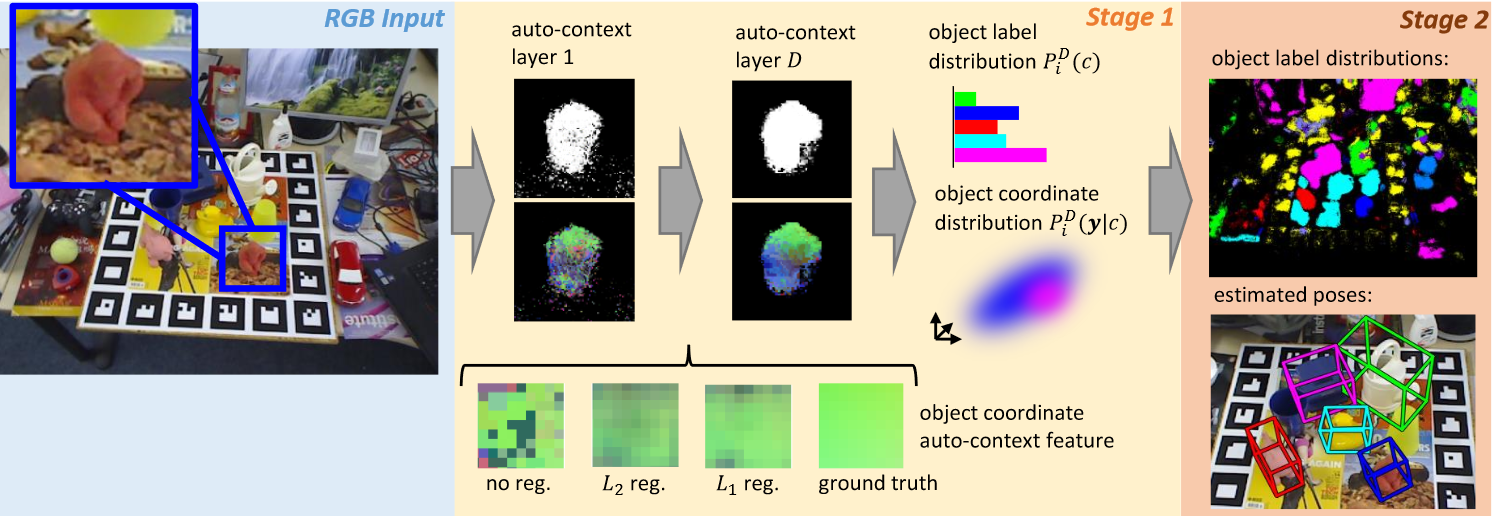
\includegraphics{Pictures/figure2.png}
\caption{Overview of the Brachmann \emph{et al.} Method}
\end{figure}

This algorithm predicts object coordinates and labels with a modified
random forest called a joint classification regression forest. This
forest is trained by mapping object coordinates to a smaller set of
discrete values using nearest neighbor assignment to the training data's
object coordinates randomly.Then those with the most information gain
when compared with the object distribution are chosen and these are
stored as a Gaussian Mixture Model. When testing an image, a pixel is
fed through a tree in the forest and when it gets to a leaf it will
store the distribution of object coordinates and predictions for that
pixel. Then all of that tree's object predictions are merged to form an
overall prediction for that pixel. The coordinate distribution for the
tree is then averaged \autocite{brachmann}.

Then Brachmann \emph{et al.} use a stack of these forests to generate
context information for each pixel in the input image. The first level
of this stack of forests is trained normally, but all the following
trees have access to the outputted information of the previous tree. To
smooth the object probability distribution they use a median filter on
the pixels surrounding each pixel. This median filter optimizes loss,
specifically the least absolute deviations that minimize the difference
between hypothesized values and target values, which allows it to be
effective when dealing with outlier pixels that would otherwise
negatively impact the result. The object coordinates are also
regularized using a similar method which optimizes
loss\autocite{brachmann}.

The object poses are then estimated using RANSAC. When RANSAC is
mentioned in this paper it is actually a specific paradigm of RANSAC
called preemptive RANSAC which estimates a certain number of hypotheses
at once. This paradigm speeds up the normal RANSAC calculation when
there are less inliers and many more outliers. Preemptive RANSAC is
better for this case since there are always a large amount of outliers,
but not too many to find a valid hypothesis. To perform this operation
for a single object the forest values of object predictions, pixel
positions, and object coordinates are used to estimate the 2D-3D
correspondences. Then the reprojection error is calculated and
subsequently minimized with the help of a camera matrix. This error is
acceptable if it is under a predefined threshold, meaning that this data
point is an inlier. The best pose hypothesis is the one in which the
largest amount of inliers are found \autocite{brachmann}. The equation
from the paper that accomplishes this task is reprinted below with the
permission of the author.

\begin{figure}
\centering
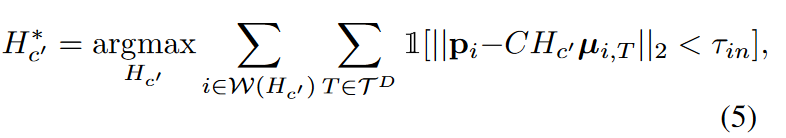
\includegraphics{Pictures/eq5.png}
\caption{The RANSAC formula to maximize inlier count of a given pose}
\end{figure}

Hypotheses are drawn by solving the perspective-n-point problem for four
correspondences. The first of four pixels is drawn according to a random
tree's mean probability distribution then the other three are drawn
within a certain distance of the first pixel depending on the size of
the object in question, but if the reprojection error calculated for the
pixels is found to be above the threshold then this hypothesis is
discarded and a new one is drawn. These hypotheses are sorted by their
number of included inliers and the lower half is discarded. The
hypotheses left after this process are then further refined by repeating
the process of solving the perspective-n-point problem on the new set of
inlier value points until only one hypothesis is left. This remaining
hypothesis is the estimated pose for the object in question
\autocite{brachmann}.

When this algorithm is detecting multiple objects at once the above
method of detection does not maintain efficiency when a large number of
objects are to be detected. Multi-object detections are performed by
drawing a shared set of hypotheses instead of individual sets for each
object. These hypotheses are chosen by analyzing the object probability
distributions at the first pixel of the current hypothesis when
performing the same actions as a single-object RANSAC pose estimation.
These chosen hypotheses still have to pass the same validity check as in
single-object detections. Using this method allows the algorithm to
decide if a hypothesis belongs to multiple objects during the hypothesis
sampling process instead of having a separate process for each object.
This allows their RANSAC pose estimation to scale more easily with a
large number of object detections in the same image
\autocite{brachmann}.

During the pose refinement stage of this implementation they replace the
standard error calculation that uses depth information with an error
based on the projection volume of a pixel. This is one of the tweaks
that allows this method to be extended to RGB images without depth
information available. Instead of calculating the log-likelihood of of
the correspondences observed in a hypothesis using the depth-based error
they find the approximate likelihood of the projection volume, as seen
in the equation seen below which was reprinted with the author's
permission, and take the log-likelihood of that \autocite{brachmann}.
Results of some final poses from the Hinterstoisser \emph{et al.}
dataset are shown in the paper's figure 4 pictured below, with
permission from both Hinterstoisser and Brachmann
\autocites{brachmann}{hinterstoisser}.

\begin{figure}
\centering
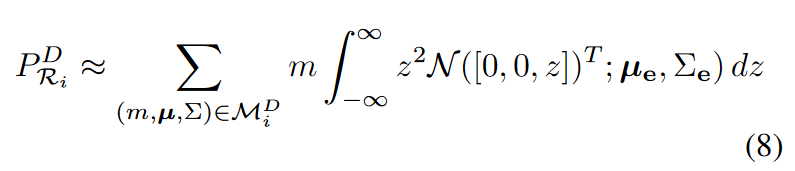
\includegraphics{Pictures/eq8.png}
\caption{Equation for projection volume approximation}
\end{figure}

\begin{figure}
\centering
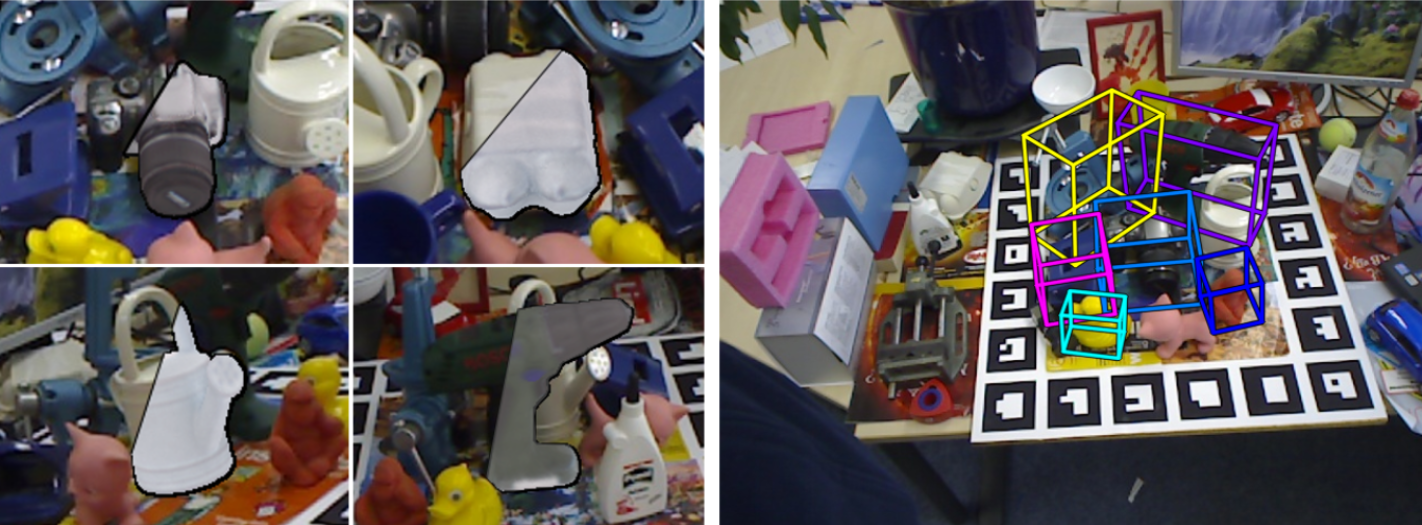
\includegraphics{Pictures/figure4.png}
\caption{Pose Overlays}
\end{figure}

Since source code and documentation were included with this paper we
have decided to use it to test the speed and accuracy of this type of
pose estimation algorithm. We will test on the smaller dataset included
with the source code (dubbed the `Dummy Data') to ensure that the
implementation is functioning correctly. Then it will be trained on the
full Asian Conference for Computer Vision (ACCV) object dataset provided
by Hinterstoisser \emph{et al.} \autocite{hinterstoisser}. Finally, we
will test this algorithm on data we collect with the Intel® RealSense™
F200 camera. We will try to match the performance metrics gathered in
this step as closely as possible when we implement a similar algorithm
in C\#.

\subsubsection{Datasets}\label{datasets}

\paragraph{The RGB-D Object Dataset}\label{the-rgb-d-object-dataset}

This dataset contains 300 objects placed into 51 different categories.
It was created with a Microsoft Kinect camera which is very similar to
the Intel® RealSense™ F200 camera we plan to use for our application.
The RGB frames are captured with width of 640 pixels and height of 480
pixels. The corresponding depth frames are captured at a rate of 30 Hz.
The data was captured by recording objects rotating 360 degrees on a
spinning table. There is pose-based ground truth data for every object
in this dataset.

This dataset also includes 22 videos of indoor scenes including the
objects in the dataset with sufficient cluttering and occlusion for our
training purposes. The varying distances in the scenes can help with
robust training for different camera setups as well \autocite{rgbdObj}.

\subsubsection{The Object Segmentation Database
(OSD)}\label{the-object-segmentation-database-osd}

The Object Segmentation Database includes data on 111 objects with
corresponding RGB-D data divided into appropriate categories based on
their basic shapes. There are categories for boxes, stacked boxes,
occlusion, cylindrical objects, mixed objects, and complex scenes. The
basic shapes provided could be an excellent resource for testing our
algorithm since the blocks provided by our sponsors are the same basic
shapes as those included in this database \autocite{osd}.

\subsubsection{Willow and Challenge
Dataset}\label{willow-and-challenge-dataset}

The Willow dataset contains 24 series of 353 total RGB-D images with
available ground-truth information and separate sets for training and
testing. These include 110 objects and 1168 appearances of those
objects.

The Challenge dataset is available alongside the Willow dataset. It
includes 39 frame sequences, with 176 RGB-D images total. These include
97 objects with 434 appearances \autocite{willowChallenge}.

\paragraph{Big Berkeley Instance Recognition Dataset (Big
BIRD)}\label{big-berkeley-instance-recognition-dataset-big-bird}

This dataset includes 600 images, 600 RGB-D-based point clouds, pose
information for every image and point cloud, segmentation masks for all
images, and meshes created from merged point clouds. This dataset is
extensive but utilizes point clouds which would not be applicable for
our purposes. Although, if extra data is needed, this could be a
potentially useful resource \autocite{bigBird}.

\paragraph{\texorpdfstring{Hinterstoisser \emph{et al.} ACCV
Dataset}{Hinterstoisser et al. ACCV Dataset}}\label{hinterstoisser-et-al.-accv-dataset}

This dataset was created for a paper presented at the Asian Conference
for Computer Vision (ACCV) by Hinterstoisser \emph{et al.}. This dataset
contains 15 videos of 15 different objects with texture-less models for
matching. There are corresponding ground truth poses for all scenes and
objects. There is sufficient variation in clutter, camera angle, camera
tilt, scene scale, and object rotation in the scenes for robust pose
estimation testing. Every video is comprised of over 1100 images from
varying angles \autocite{hinterstoisser}. This dataset is used to test
the method presented in ``Uncertainty-Driven 6D Pose Estimation of
Objects and Scenes from a Single RGB Image'' and we would like to test
our implementation on this dataset to benchmark test our implementation
against the one presented by Brachmann \emph{et al}
\autocite{brachmann}.

\subsection{Unity Game Engine
Research}\label{unity-game-engine-research}

\subsubsection{Basic Unity}\label{basic-unity}

\paragraph{Overview}\label{overview-1}

Unity is a game development engine that permits users to create a
variety of games for different platforms, some of the biggest being PC,
Xbox, Playstation, and Android/IOS.\\
The base requirements for Unity version 5.5.0 are:

OS: Windows 7 SP1+, 8, 10; Mac OSX 10.8+ GPU: Graphics card with DX9
(shader model 3.0) or DX11 with feature level 9.3 capabilities

\paragraph{Scripting}\label{scripting}

Unity uses an implementation of the Mono runtime for scripting. Mono is
an implementation of the .NET framework. Mono is sponsored by Microsoft
and it follows the ECMA standards for C\#.

Unity mainly supports two scripting languages, C\# (which is what this
project is using) and UnityScript, which is a language that is modelled
after Javascript to use specifically for Unity. Unity can compile the
source code that is in the ``Assets'' folder of the project. For other
languages, they can be used in Unity scripts in the form of DLLs, so as
long as a language can be compiled into a Dynamically Linked
Library(DLL) file it can be tied into Unity scripts.

Unity's GameObjects are controlled by Components that are attached to
them, and scripts allow the user to create these Components and
manipulate them dynamically. Unity's GUI allows for a simple script
creation by going to Assets -\textgreater{} Create -\textgreater{} C\#
Script or Assets -\textgreater{} Create -\textgreater{} Javascript. This
will create a class following your naming convention that extends
MonoBehaviour and has two methods already created,
\texttt{void\ Start()} and \texttt{void\ Update()}.

The extension of MonoBehavior is necessary to allow the script to
interface with Unity. It contains the necessary classes to allow for the
created script to affect the GameObjects in Unity. It also gives the
class access to the functions that determine when the script is called
(like start and update). The \texttt{Start()} method is called by Unity
when the script is initialized, whereas the \texttt{Update()} method is
called by Unity on every frame of the game. \autocite{unityScripts}

\paragraph{3D Models}\label{d-models}

Unity has two kinds of file that it can use to import 3D models. The
first is exported 3D file formats and the second is application files
from 3D Editors.

The exported 3D file formats that Unity uses are: .FBX, .dxf, .obj,
.3DS, and.dae. The benefit to these kinds of files are that they tend to
be smaller than the application files and export only the data you will
be using. These types of files are more generalized and are more easily
generated programatically due to them not being proprietary to a certain
piece of premium software.

The applications that unity accepts files from are: Blender, Cinema4D,
Cheetah3D, Lightwave, Maya, Max, and Modo. These kinda of files tend to
be simpler in terms of usability, especially since Unity will re-import
the model every time the user saves the file. But they also tend to be
larger when compared with exported files due to data bloating which is
commonly found within 3D modeling software, which can cause a slowdown
of Unity. The proprietary software used to create the file must also be
owned and licensed on the computer in which it's being used.

Unity itself has support for simple models to be created through the
editor. In the main editor screen, the user can go to Create
-\textgreater{} 3D Objects and choose from a list of different simple 3D
objects such as cubes or cylinders. Unity will then spawn the object,
typically at world coordinates (0, 0, 0), and the user can edit them.

Unity also also has support for dynamic Mesh creation.

The file format for 3D models we have chosen to use for our project in
the Unity Engine is the .obj format mentioned previously. This format
was chosen due to some key advantages such as the ability to generate
the file programatically if it is found to be necessary. The .obj file
specification is also publicly available and allows us to construct .obj
files from scratch. The four types of vertex types are geometric
vertices (\texttt{v}), texture vertices (\texttt{vt}), vertex normals
(\texttt{vn}), and parameter space vertices (\texttt{vp})
\autocite{obj}.

The following are proper syntax examples in the .obj file format:

\texttt{v\ x\ y\ z\ w} for a geometric vertex, where \texttt{x},
\texttt{y}, and \texttt{z} are coordinates of a vertex and \texttt{w} is
a weight for curves defaulted to one.

\texttt{vp\ u\ v\ w} for a freeform geometry, where \texttt{u} is either
a coordinate of a curve or the first coordinate of a surface. \texttt{v}
is the second coordinate of a surface. \texttt{w} is a curve trimming
weight defaulted to one.

\texttt{vn\ i\ j\ k} for a normal vertex, where \texttt{i}, \texttt{j},
and \texttt{k} are the normal vector components.

\texttt{vt\ u\ v\ w} for a texture vertex, where \texttt{u} is the
horizontal direction, \texttt{v} is the vertical direction , and
\texttt{w} is the depth. Depending on the dimensionality of the texture,
\texttt{u} and \texttt{v} may be 0.

Syntax for different geometric elements are as follows:

\texttt{p\ v1\ v2\ ...\ vn} for a point, where \texttt{vn} represents
the nth vertex which will create the nth point.

\texttt{l\ v1/vt1\ v2/vt2\ ...\ vn/vtn} for a line, where
\texttt{vn/vtn} represents the nth vertex on the line separated from the
texture vertex with a \texttt{/}.

\texttt{f\ v1/vt1/vn1\ v2/vt2/vn2\ ...\ vn/vtn/vnn} for a face, where
\texttt{vn/vtn/vnn} represents the nth vertex, texture vertex, and
normal vertex respectively.

\texttt{curv\ u0\ u1\ v1\ v2\ ...\ vn} for a curve, where \texttt{u0} is
a float representing the starting parameter value for the curve,
\texttt{u1} is a float representing the ending parameter value for the
curve, and \texttt{vn} represents the nth control point parameter vertex
for the curve (there must be at least two).

\texttt{curv2\ vp1\ ...\ vpn} for a 2D curve, where \texttt{vpn} is the
nth control point parameter vertices.

\texttt{surf\ s0\ s1\ t0\ t1\ v1/vt1/vn1\ ...\ vn/vtn/vnn} for a
surface, where \texttt{s0} is the start parameter value for the u
direction, \texttt{s1} is the end parameter value for the u direction,
\texttt{t0} is the start parameter value for the v direction,
\texttt{t1} is the end parameter value for the v direction and
\texttt{vn/vtn/vnn} is the nth control vertex with the nth texture
vertex and normal vertex separated by a \texttt{/} \autocite{obj}.

\paragraph{Asset Store}\label{asset-store}

Unity has an Asset Store where users can put any plugins that they
create to be sold to other Unity users. It contains thousands of plugins
and other assets created by thousands of users for use in a large amount
of game types. From 3D to 2D, controls, sprites, models, and more it can
all be found on the Unity asset store. some of these assets are free for
anyone's use and others have to be paid for. Any Unity user with an
account can have their assets looked at by a Unity Assets Store team and
then placed on the asset store for purchase.

\subsubsection{Plugin types}\label{plugin-types}

\paragraph{Managed Plugins}\label{managed-plugins}

Managed plugins are a type of plugin that Unity supports which allows
Unity to use C\# code that has been created by a third party to
supplement created code. It allows for a community to form around Unity
that continuously builds additional functionality allowing users to
create better products. Many Unity users eventually will place their
managed plugins on the Unity Asset store for others to buy and then
use/improve on for their needs.

Unity allows for any C\# files in a folder labeled ``plugins'' under the
Assets folder to be considered a plugin, the files in that folder will
be included with every C\# script that the user creates, allowing access
to the methods.

Managed plugins can also be implemented through the usage of Dynamically
Linked Libraries (DLLs). This allows a user to take C\# code and compile
it through a different compiler into a DLL, then the user can place the
DLL into a unity plugin folder to be used in their scripts. from there
the DLLs can be used in the same way that normal C\# scripts are used in
Unity. \autocite{unityManaged}

\paragraph{Native Plugins}\label{native-plugins}

Native plugins are libraries of native code that is written in any
language that is not directly compiled by Unity, that can also be
compiled into a DLL (Windows). The process of placing the Native Plugin
into the project is the same as Managed Plugins, you create a folder
titled ``plugins'' located under the Assets folder and drop the DLLs in
there.

To access the methods or functions from the DLL files the user must add
tags on the C\# method used to call the DLL method. First you import the
plugin, then you can declare the external method using the extern
modifier to mark it as an external function:

\texttt{{[}DllImport\ ("PluginName"){]}}

\texttt{private\ static\ extern\ pFunction();}

The user can then use the declared method to make a call to the native
method/function from the DLL. It should be noted that when creating
Native Plugins using C++ or Objective-C, there must be steps taken to
avoid name mangling issues, because plugin functions use a C-based call
interface.

Any version of Unity that is below 5 requires either a Unity Pro License
or a Unity Enterprise License to be able to use Native Plugins. Unity 5,
however, allows all versions to use Native Plugins, from the Personal
version to the Enterprise Version. \autocite{unityNative}

\paragraph{Extending the Editor (Maybe change this part's
location)}\label{extending-the-editor-maybe-change-this-parts-location}

Similarly to how plugins can be made for game logic in Unity, one could
also create plugins to extends the Unity editor itself to make game
functionality easier. In fact, one might say that is the entire purpose
of this project. To extend the editor, a script needs to be created
where the class extends EditorWindow. This script will create a new
editor window

\subsubsection{Version Differences and
Pricing}\label{version-differences-and-pricing}

\begin{longtable}[]{@{}ccccc@{}}
\toprule
\begin{minipage}[b]{0.18\columnwidth}\centering\strut
Features\strut
\end{minipage} & \begin{minipage}[b]{0.18\columnwidth}\centering\strut
Personal\strut
\end{minipage} & \begin{minipage}[b]{0.14\columnwidth}\centering\strut
Plus\strut
\end{minipage} & \begin{minipage}[b]{0.14\columnwidth}\centering\strut
Pro\strut
\end{minipage} & \begin{minipage}[b]{0.23\columnwidth}\centering\strut
Enterprise\strut
\end{minipage}\tabularnewline
\midrule
\endhead
\begin{minipage}[t]{0.18\columnwidth}\centering\strut
All Engine Features\strut
\end{minipage} & \begin{minipage}[t]{0.18\columnwidth}\centering\strut
Y\strut
\end{minipage} & \begin{minipage}[t]{0.14\columnwidth}\centering\strut
Y\strut
\end{minipage} & \begin{minipage}[t]{0.14\columnwidth}\centering\strut
Y\strut
\end{minipage} & \begin{minipage}[t]{0.23\columnwidth}\centering\strut
Y\strut
\end{minipage}\tabularnewline
\begin{minipage}[t]{0.18\columnwidth}\centering\strut
All Platforms\strut
\end{minipage} & \begin{minipage}[t]{0.18\columnwidth}\centering\strut
Y\strut
\end{minipage} & \begin{minipage}[t]{0.14\columnwidth}\centering\strut
Y\strut
\end{minipage} & \begin{minipage}[t]{0.14\columnwidth}\centering\strut
Y\strut
\end{minipage} & \begin{minipage}[t]{0.23\columnwidth}\centering\strut
Y\strut
\end{minipage}\tabularnewline
\begin{minipage}[t]{0.18\columnwidth}\centering\strut
Continuous Updates\strut
\end{minipage} & \begin{minipage}[t]{0.18\columnwidth}\centering\strut
Y\strut
\end{minipage} & \begin{minipage}[t]{0.14\columnwidth}\centering\strut
Y\strut
\end{minipage} & \begin{minipage}[t]{0.14\columnwidth}\centering\strut
Y\strut
\end{minipage} & \begin{minipage}[t]{0.23\columnwidth}\centering\strut
Y\strut
\end{minipage}\tabularnewline
\begin{minipage}[t]{0.18\columnwidth}\centering\strut
Royalty Free\strut
\end{minipage} & \begin{minipage}[t]{0.18\columnwidth}\centering\strut
Y\strut
\end{minipage} & \begin{minipage}[t]{0.14\columnwidth}\centering\strut
Y\strut
\end{minipage} & \begin{minipage}[t]{0.14\columnwidth}\centering\strut
Y\strut
\end{minipage} & \begin{minipage}[t]{0.23\columnwidth}\centering\strut
Y\strut
\end{minipage}\tabularnewline
\begin{minipage}[t]{0.18\columnwidth}\centering\strut
Splash Screen\strut
\end{minipage} & \begin{minipage}[t]{0.18\columnwidth}\centering\strut
Y\strut
\end{minipage} & \begin{minipage}[t]{0.14\columnwidth}\centering\strut
Custom\strut
\end{minipage} & \begin{minipage}[t]{0.14\columnwidth}\centering\strut
Custom\strut
\end{minipage} & \begin{minipage}[t]{0.23\columnwidth}\centering\strut
Custom\strut
\end{minipage}\tabularnewline
\begin{minipage}[t]{0.18\columnwidth}\centering\strut
Revenue Capacity\strut
\end{minipage} & \begin{minipage}[t]{0.18\columnwidth}\centering\strut
\$100k\strut
\end{minipage} & \begin{minipage}[t]{0.14\columnwidth}\centering\strut
\$200k\strut
\end{minipage} & \begin{minipage}[t]{0.14\columnwidth}\centering\strut
Unlimited\strut
\end{minipage} & \begin{minipage}[t]{0.23\columnwidth}\centering\strut
Unlimited\strut
\end{minipage}\tabularnewline
\begin{minipage}[t]{0.18\columnwidth}\centering\strut
Unity Cloud Build\strut
\end{minipage} & \begin{minipage}[t]{0.18\columnwidth}\centering\strut
Standard Queue\strut
\end{minipage} & \begin{minipage}[t]{0.14\columnwidth}\centering\strut
Priority Queue\strut
\end{minipage} & \begin{minipage}[t]{0.14\columnwidth}\centering\strut
Concurrent Builds\strut
\end{minipage} & \begin{minipage}[t]{0.23\columnwidth}\centering\strut
Dedicated Build Agents\strut
\end{minipage}\tabularnewline
\begin{minipage}[t]{0.18\columnwidth}\centering\strut
Unity Analytics\strut
\end{minipage} & \begin{minipage}[t]{0.18\columnwidth}\centering\strut
Personal Analytics\strut
\end{minipage} & \begin{minipage}[t]{0.14\columnwidth}\centering\strut
Plus Analytics\strut
\end{minipage} & \begin{minipage}[t]{0.14\columnwidth}\centering\strut
Pro Analytics\strut
\end{minipage} & \begin{minipage}[t]{0.23\columnwidth}\centering\strut
Custom Analytics\strut
\end{minipage}\tabularnewline
\begin{minipage}[t]{0.18\columnwidth}\centering\strut
Unity Multiplayer\strut
\end{minipage} & \begin{minipage}[t]{0.18\columnwidth}\centering\strut
20 Concurrent Users\strut
\end{minipage} & \begin{minipage}[t]{0.14\columnwidth}\centering\strut
50 Concurrent Users\strut
\end{minipage} & \begin{minipage}[t]{0.14\columnwidth}\centering\strut
200 Concurrent Users\strut
\end{minipage} & \begin{minipage}[t]{0.23\columnwidth}\centering\strut
Custom Multiplayer\strut
\end{minipage}\tabularnewline
\begin{minipage}[t]{0.18\columnwidth}\centering\strut
Unity Ads\strut
\end{minipage} & \begin{minipage}[t]{0.18\columnwidth}\centering\strut
Y\strut
\end{minipage} & \begin{minipage}[t]{0.14\columnwidth}\centering\strut
Y\strut
\end{minipage} & \begin{minipage}[t]{0.14\columnwidth}\centering\strut
Y\strut
\end{minipage} & \begin{minipage}[t]{0.23\columnwidth}\centering\strut
Y\strut
\end{minipage}\tabularnewline
\begin{minipage}[t]{0.18\columnwidth}\centering\strut
Beta Access\strut
\end{minipage} & \begin{minipage}[t]{0.18\columnwidth}\centering\strut
Y\strut
\end{minipage} & \begin{minipage}[t]{0.14\columnwidth}\centering\strut
Y\strut
\end{minipage} & \begin{minipage}[t]{0.14\columnwidth}\centering\strut
Y\strut
\end{minipage} & \begin{minipage}[t]{0.23\columnwidth}\centering\strut
Y\strut
\end{minipage}\tabularnewline
\begin{minipage}[t]{0.18\columnwidth}\centering\strut
Pro Editor UI Skin\strut
\end{minipage} & \begin{minipage}[t]{0.18\columnwidth}\centering\strut
N\strut
\end{minipage} & \begin{minipage}[t]{0.14\columnwidth}\centering\strut
Y\strut
\end{minipage} & \begin{minipage}[t]{0.14\columnwidth}\centering\strut
Y\strut
\end{minipage} & \begin{minipage}[t]{0.23\columnwidth}\centering\strut
Y\strut
\end{minipage}\tabularnewline
\begin{minipage}[t]{0.18\columnwidth}\centering\strut
Performance Reporting\strut
\end{minipage} & \begin{minipage}[t]{0.18\columnwidth}\centering\strut
N\strut
\end{minipage} & \begin{minipage}[t]{0.14\columnwidth}\centering\strut
Y\strut
\end{minipage} & \begin{minipage}[t]{0.14\columnwidth}\centering\strut
Y\strut
\end{minipage} & \begin{minipage}[t]{0.23\columnwidth}\centering\strut
Y\strut
\end{minipage}\tabularnewline
\begin{minipage}[t]{0.18\columnwidth}\centering\strut
Flexible Seat Management\strut
\end{minipage} & \begin{minipage}[t]{0.18\columnwidth}\centering\strut
N\strut
\end{minipage} & \begin{minipage}[t]{0.14\columnwidth}\centering\strut
Y\strut
\end{minipage} & \begin{minipage}[t]{0.14\columnwidth}\centering\strut
Y\strut
\end{minipage} & \begin{minipage}[t]{0.23\columnwidth}\centering\strut
Y\strut
\end{minipage}\tabularnewline
\begin{minipage}[t]{0.18\columnwidth}\centering\strut
Asset Kits\strut
\end{minipage} & \begin{minipage}[t]{0.18\columnwidth}\centering\strut
N\strut
\end{minipage} & \begin{minipage}[t]{0.14\columnwidth}\centering\strut
20\% Off\strut
\end{minipage} & \begin{minipage}[t]{0.14\columnwidth}\centering\strut
40\% off\strut
\end{minipage} & \begin{minipage}[t]{0.23\columnwidth}\centering\strut
40\% off\strut
\end{minipage}\tabularnewline
\begin{minipage}[t]{0.18\columnwidth}\centering\strut
Unity Certification Courseware\strut
\end{minipage} & \begin{minipage}[t]{0.18\columnwidth}\centering\strut
N\strut
\end{minipage} & \begin{minipage}[t]{0.14\columnwidth}\centering\strut
1 Month Access\strut
\end{minipage} & \begin{minipage}[t]{0.14\columnwidth}\centering\strut
3 Month Access\strut
\end{minipage} & \begin{minipage}[t]{0.23\columnwidth}\centering\strut
3 Month Access\strut
\end{minipage}\tabularnewline
\begin{minipage}[t]{0.18\columnwidth}\centering\strut
Source Code Access\strut
\end{minipage} & \begin{minipage}[t]{0.18\columnwidth}\centering\strut
N\strut
\end{minipage} & \begin{minipage}[t]{0.14\columnwidth}\centering\strut
N\strut
\end{minipage} & \begin{minipage}[t]{0.14\columnwidth}\centering\strut
\$\strut
\end{minipage} & \begin{minipage}[t]{0.23\columnwidth}\centering\strut
\$\strut
\end{minipage}\tabularnewline
\begin{minipage}[t]{0.18\columnwidth}\centering\strut
Premium Support\strut
\end{minipage} & \begin{minipage}[t]{0.18\columnwidth}\centering\strut
N\strut
\end{minipage} & \begin{minipage}[t]{0.14\columnwidth}\centering\strut
N\strut
\end{minipage} & \begin{minipage}[t]{0.14\columnwidth}\centering\strut
\$\strut
\end{minipage} & \begin{minipage}[t]{0.23\columnwidth}\centering\strut
\$\strut
\end{minipage}\tabularnewline
\bottomrule
\end{longtable}

\autocite{unityTable}

\paragraph{Unity free}\label{unity-free}

Unity Free is the base version of Unity that anyone can download from
their website at www.unity3d.com. The base requirements for Unity
version 5.5.0 are:

OS: Windows 7 SP1+, 8, 10; Mac OSX 10.8+ GPU: Graphics card with DX9
(shader model 3.0) or DX11 with feature level 9.3 capabilities

Unity's base edition is different from the other editions in a variety
of ways. Any game created in it automatically has a short splash screen
video play at the beginning of any game when it is launched depicting
the Unity logo with the words ``Personal Edition'' under the logo.

Unity personal comes with a \$100k revenue capacity. What that means is
that if an entity uses Unity personal to create their game and then
sells it, if the game makes more than \$100,000 dollars in annual gross
revenue, that entity must sign up for either the Plus, Pro, or
Enterprise edition of Unity. If they do not, then they are not allowed
to use Unity anymore. They may still sell the game which made them that
money, but they are no longer allowed to update or expand that game at
all, or make any new games using Unity.

The personal edition also comes with the Unity Cloud Build feature, it
allows developers to instantly compile, test, and deploy the game builds
to everyone that needs it. The standard queue processes the builds in
FIFO form across all Unity customers.

Unity Analytics is a feature that allows game developers seamlessly view
information about their game like how it's being used, general gameplay
behaviors, and it comes with a money optimization feature. It comes with
Unity IAP, which allows users to set up In-App Purchases within their
game and keep track of it across all platforms. \autocite{unityTable}

\paragraph{Unity Plus}\label{unity-plus}

Unity Plus is the version of Unity that is one level above the personal
edition. It costs \$35 per person per month and comes with upgraded
features.

The first upgraded feature is the splash screen. The Plus edition allows
users to either use the normal Unity splash screen, create their own
splash screen and insert it into where the Unity splash screen would be,
or elect to not use a splash screen at all.

The Plus edition also upgrades the revenue capacity by \$100k extra,
allowing users to make an annual gross revenue of \$200k before they are
required to either subscribe for Unity Pro Edition or Unity Enterprise
Edition.

The Unity Cloud Build feature is also improved in the plus version, it
gives the user a Priority Queue allowing their builds to be compiled,
tested, and deployed faster than the personal version queue.

Unity Plus gives users access to all the features in Unity Analytics
that the personal version users have, but also gives Priority Analytics,
livestream support, and more specific analysis of the game data.

Unity Plus also comes with a dark theme called the Pro Editor UI theme
which is not available for the personal version.

Performance reporting is a feature that is only available in Unity Plus
and above. It allows users to view bugs and errors in all of their Unity
builds across all platforms, it prioritizes issues as they are reported
in realtime.

Another feature that Unity Plus has is Flexible Seat Management, this
allows a moderator/manager of the entity or team that uses Unity to
control what person on the team uses Unity and how they use it.

Another thing that having a Plus subscription gives users is a 20\%
discount in the Unity Assets Store, plus one months access to Unity's
Certification Program. \autocite{unityTable}

\paragraph{Unity Pro}\label{unity-pro}

Unity Pro edition is the next tier of Unity above the Unity Plus
Edition. It costs \$125 per person per month and upgrades the features
even more than Unity Plus does. Unity pro contains all of the features
that the previous two have, with some upgrades.

Unity Pro edition has no limit on revenue like the previous versions.
Anyone who is subscribed to the pro version can make any Unity game and
does not have to change their subscription based on how much they make.
This is most likely because Unity Pro is the highest tier of Unity that
a single person can buy.

The Unity Cloud feature is upgraded further from the Plus Unity Cloud
feature. It still contains the Priority Queue allowing th user to have a
faster build time than the Personal users, but it also allows for
creating multiple parallel builds for any project.

Unity Analytics comes with the Unity Pro Analytics feature. It has all
that plus has with 50 gigabytes of raw data export. It also has even
more game data analysis than the plus version.

The Assets Store discount is upped in Pro to 40\% from the 20\% that is
discounted in Plus. The Unity Certification Course access is extended to
3 months. \autocite{unityTable}

\paragraph{Unity Enterprise}\label{unity-enterprise}

Unity's Enterprise edition is somewhat of a mix of the previous
versions. It allows businesses to make a customized plan for all of
their workers that need Unity to give those who need specific versions
exactly what they need. This also gives the business access to special
Enterprise features.

In the Enterprise tier, Unity will build a custom Unity Cloud
infrastructure to give the business a queue time that only includes the
users in that business.

The Unity Analytics feature is also upgraded in the Enterprise tier to a
level that is configurable by the business. It has all the features of
Pro with a custom raw data export size and a custom analysis.
\autocite{unityTable}

\subsection{Unreal Engine 4 Research}\label{unreal-engine-4-research}

Unity is the primary target of our project, but the Unreal Engine is
similar target that may serve as an additional implementation path. The
Unreal Engine has recently changed into a free-to-use model, with a
royalty needed if the profits exceed three thousand dollars per quarter.
This is important to note for our project because of the implications
for educational use. With that in mind, we will describe the process of
creating a similar implementation of our project in the Unreal Engine.

\subsubsection{Plugin System}\label{plugin-system}

Unlike Unity, Unreal plugins operate on a relatively separate layer of
engine itself. The support documentation for the system is also sparse,
due to the relatively new implementation of the system (2015).

Unreal uses C++ within its environment to do programming, and the same
goes for the plugin system. For the most part, plugin source file layout
is the same as any other C++ module in Unreal Engine. The Primary
addition is a *.uplugin file that acts as a descriptor for the plugin.

\paragraph{Descriptors}\label{descriptors}

Plugin descriptors are files that end in a *.uplugin extension that are
formatted like JSON. one should refer to the following two tables to
create a proper plugin description couple with a proper proper module
description.

Descriptor File Format \autocite{unreal:plugins}

\begin{figure}
\centering
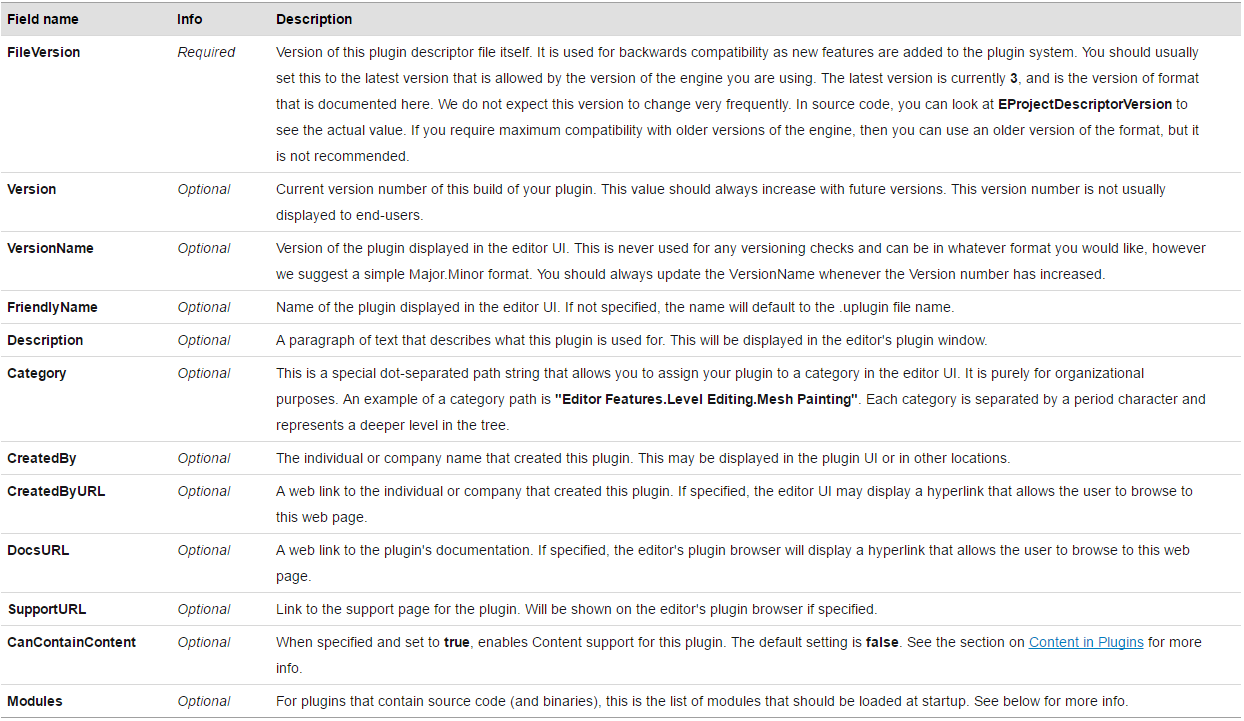
\includegraphics{Pictures/Descriptor.PNG}
\caption{Descriptor File Format}
\end{figure}

Module Descriptors \autocite{unreal:plugins}

\begin{figure}
\centering
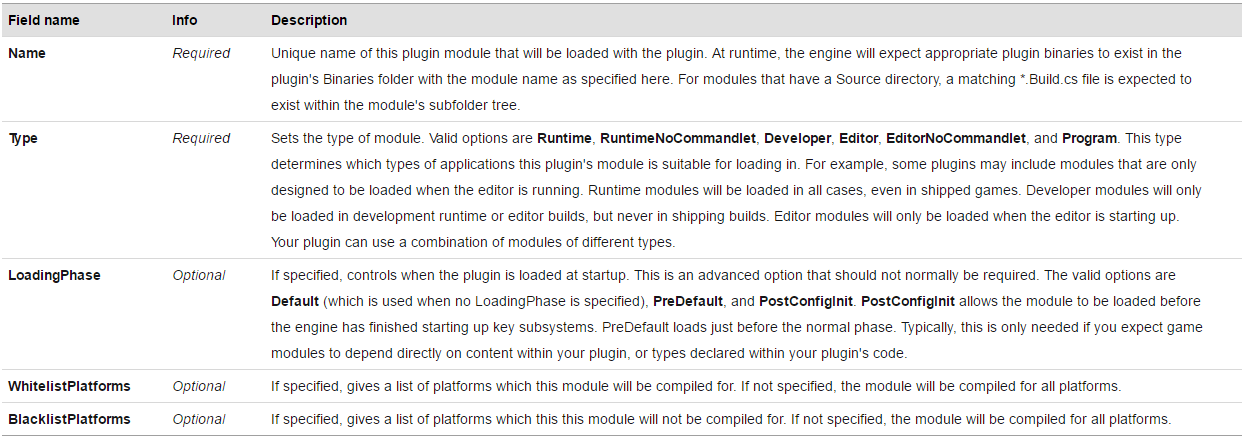
\includegraphics{Pictures/ModuleD.PNG}
\caption{Module Descriptors}
\end{figure}

\paragraph{Plugin Code}\label{plugin-code}

The process for developing our plugin in Unreal will be very similar to
the process in Unity, because we will be linking a DLL from within the
plugin to provide the necessary functions to access hardware and do the
computation algorithms. To start the process, every plugin will start
with the following two steps:

\begin{enumerate}
\def\labelenumi{\arabic{enumi}.}
\tightlist
\item
  Duplicate the template plugin folder structure given by Unreal.
\item
  Modify the Plugin and Module Descriptors to match the new plugin.
\end{enumerate}

\paragraph{DLL Import}\label{dll-import}

With a blank plugin set up, it is pertinent to note the means by which
one loads a DLL into the plugin. You will need a minimum of three
things:

\begin{enumerate}
\def\labelenumi{\arabic{enumi}.}
\tightlist
\item
  The DLL itself
\item
  The .h header file that declares all the functions of the DLL that you
  can call
\item
  The .lib file or import library which contains address of the header
  file functions in the DLL
\end{enumerate}

Once those files are collected and placed in the project, once has to
follow the next three steps to use the functions in the DLL:

\begin{enumerate}
\def\labelenumi{\arabic{enumi}.}
\item
  In the build.cs, add the following lines:

  \texttt{PublicDelayLoadDLLs.Add("FreeImage.dll");}
  \texttt{PublicAdditionalLibraries.Add(Path.Combine(FreeImageDirectory,\ "FreeImage.lib"));}
\item
  In the main cpp file for the plugin, add the following:

  \texttt{DLLHandle\ =\ FPlatformProcess::GetDllHandle(*Path);}
\end{enumerate}

After all that, just include the header in any file in the plugin and
call any of the DLL functions.

\section{Detailed Design}\label{detailed-design}

\subsection{Camera Design}\label{camera-design}

The design of the camera module strives to implement the fundamental
concept of separating interface from implementation. By defining an
\texttt{ICamera} interface that handles all public access, the
underlying implementation can change dramatically as long as it conforms
to the contract specified by the interface. This allows for supporting
additional cameras in future versions of the product as well as making
camera changes should unforeseeable events occur. All these changes can
happen within the camera module without the unity plugin needing to
change its method calls at all.

\subsubsection{ICamera Public Members}\label{icamera-public-members}

The \texttt{RealSenseCamera} has three public members. All three of its
public members are implementations of the \texttt{ICamera} interface's
public members They include: \texttt{StartCapture()},
\texttt{StopCapture()}, and \texttt{GetImages()}. Each of these public
members are described below.

\paragraph{StartCapture}\label{startcapture}

The \texttt{StartCapture} method of the \texttt{RealSenseCamera} signals
the class to start capturing images from the Intel® RealSense™ F200
Camera. This updates the camera's state variable to the
\texttt{CameraState.RUNNING} state. The method will engage the camera
capture loop which will continually capture images until otherwise
notified. This notification is created by calling the
\texttt{StopCapture} method described below.

\paragraph{StopCapture}\label{stopcapture}

The \texttt{StopCapture} method of the \texttt{RealSenseCamera} signals
the class to stop capturing images from the Intel® RealSense™ F200
Camera. The \texttt{State} member variable will be changed in order to
signal to the capture loop to terminate. The camera module will then
finish converting and saving all images that have been captured. Image
capture will not resume again until the \texttt{StartCapture} method has
been called.

\paragraph{GetImage}\label{getimage}

Gets the next available image from the camera as a \texttt{Bitmap}. If
an image is available, it will be returned. Otherwise, the function will
block if the \texttt{Status} member equals \texttt{CameraStatus.RUNNING}
and return the next available image once it becomes available. If the
\texttt{Status} member equals \texttt{CameraStatus.STOPPED}, the method
will return \texttt{null} to signal that there are no available images.

\subsubsection{Concurrency}\label{concurrency}

The ICamera Interface should be able to return a \texttt{Bitmap} image
while still capturing data. This will be accomplished by placing
captured images into a
\texttt{ConcurrentQueue\textless{}Bitmap\textgreater{}}. When the queue
reaches a certain capacity the remaining captured images will be written
to a disk. As the
\texttt{ConcurrentQueue\textless{}Bitmap\textgreater{}} empties the
images will be read from disk and loaded back into the queue. In order
to accomplish this concurrency, two threads will be needed. One thread
will be used to produce data. The other thread will belong to the caller
of the \texttt{GetImage} method and will be used to dequeue the next
image, by blocking if necessary, and serve it the caller. The only
resource shared between the two threads are the
\texttt{ConcurrentQueue\textless{}Bitmap\textgreater{}} which will
account for synchronization issues between the two.

\subsection{Computer Vision Design}\label{computer-vision-design}

\subsubsection{Accord.NET Framework}\label{accord.net-framework}

The Accord.NET framework is a machine learning framework written in C\#
for signal processing, statistics, computer audition, and computer
vision applications. Accord.NET extends AForge.NET which is another
popular C\# machine learning framework, but Accord adds extra scientific
computing features.

The libraries available in the Accord.NET framework are divided into
three sections: scientific computing, signal and image processing, and
support libraries. One primary namespace we will be using is
\texttt{Accord.MachineLearning} for \texttt{DecisionTrees},
\texttt{GaussianMixtureModel} and the RANSAC implementation included
\autocite{accord}.

Another useful namespace for this project is \texttt{Accord.Math} for
integration techniques among other mathematical implementations that
will prove useful for calculating loss minimization, refining the RANSAC
pose estimation, and any other mathematical equations we incorporate
into our implementation \autocite{accord}.

\begin{figure}
\centering
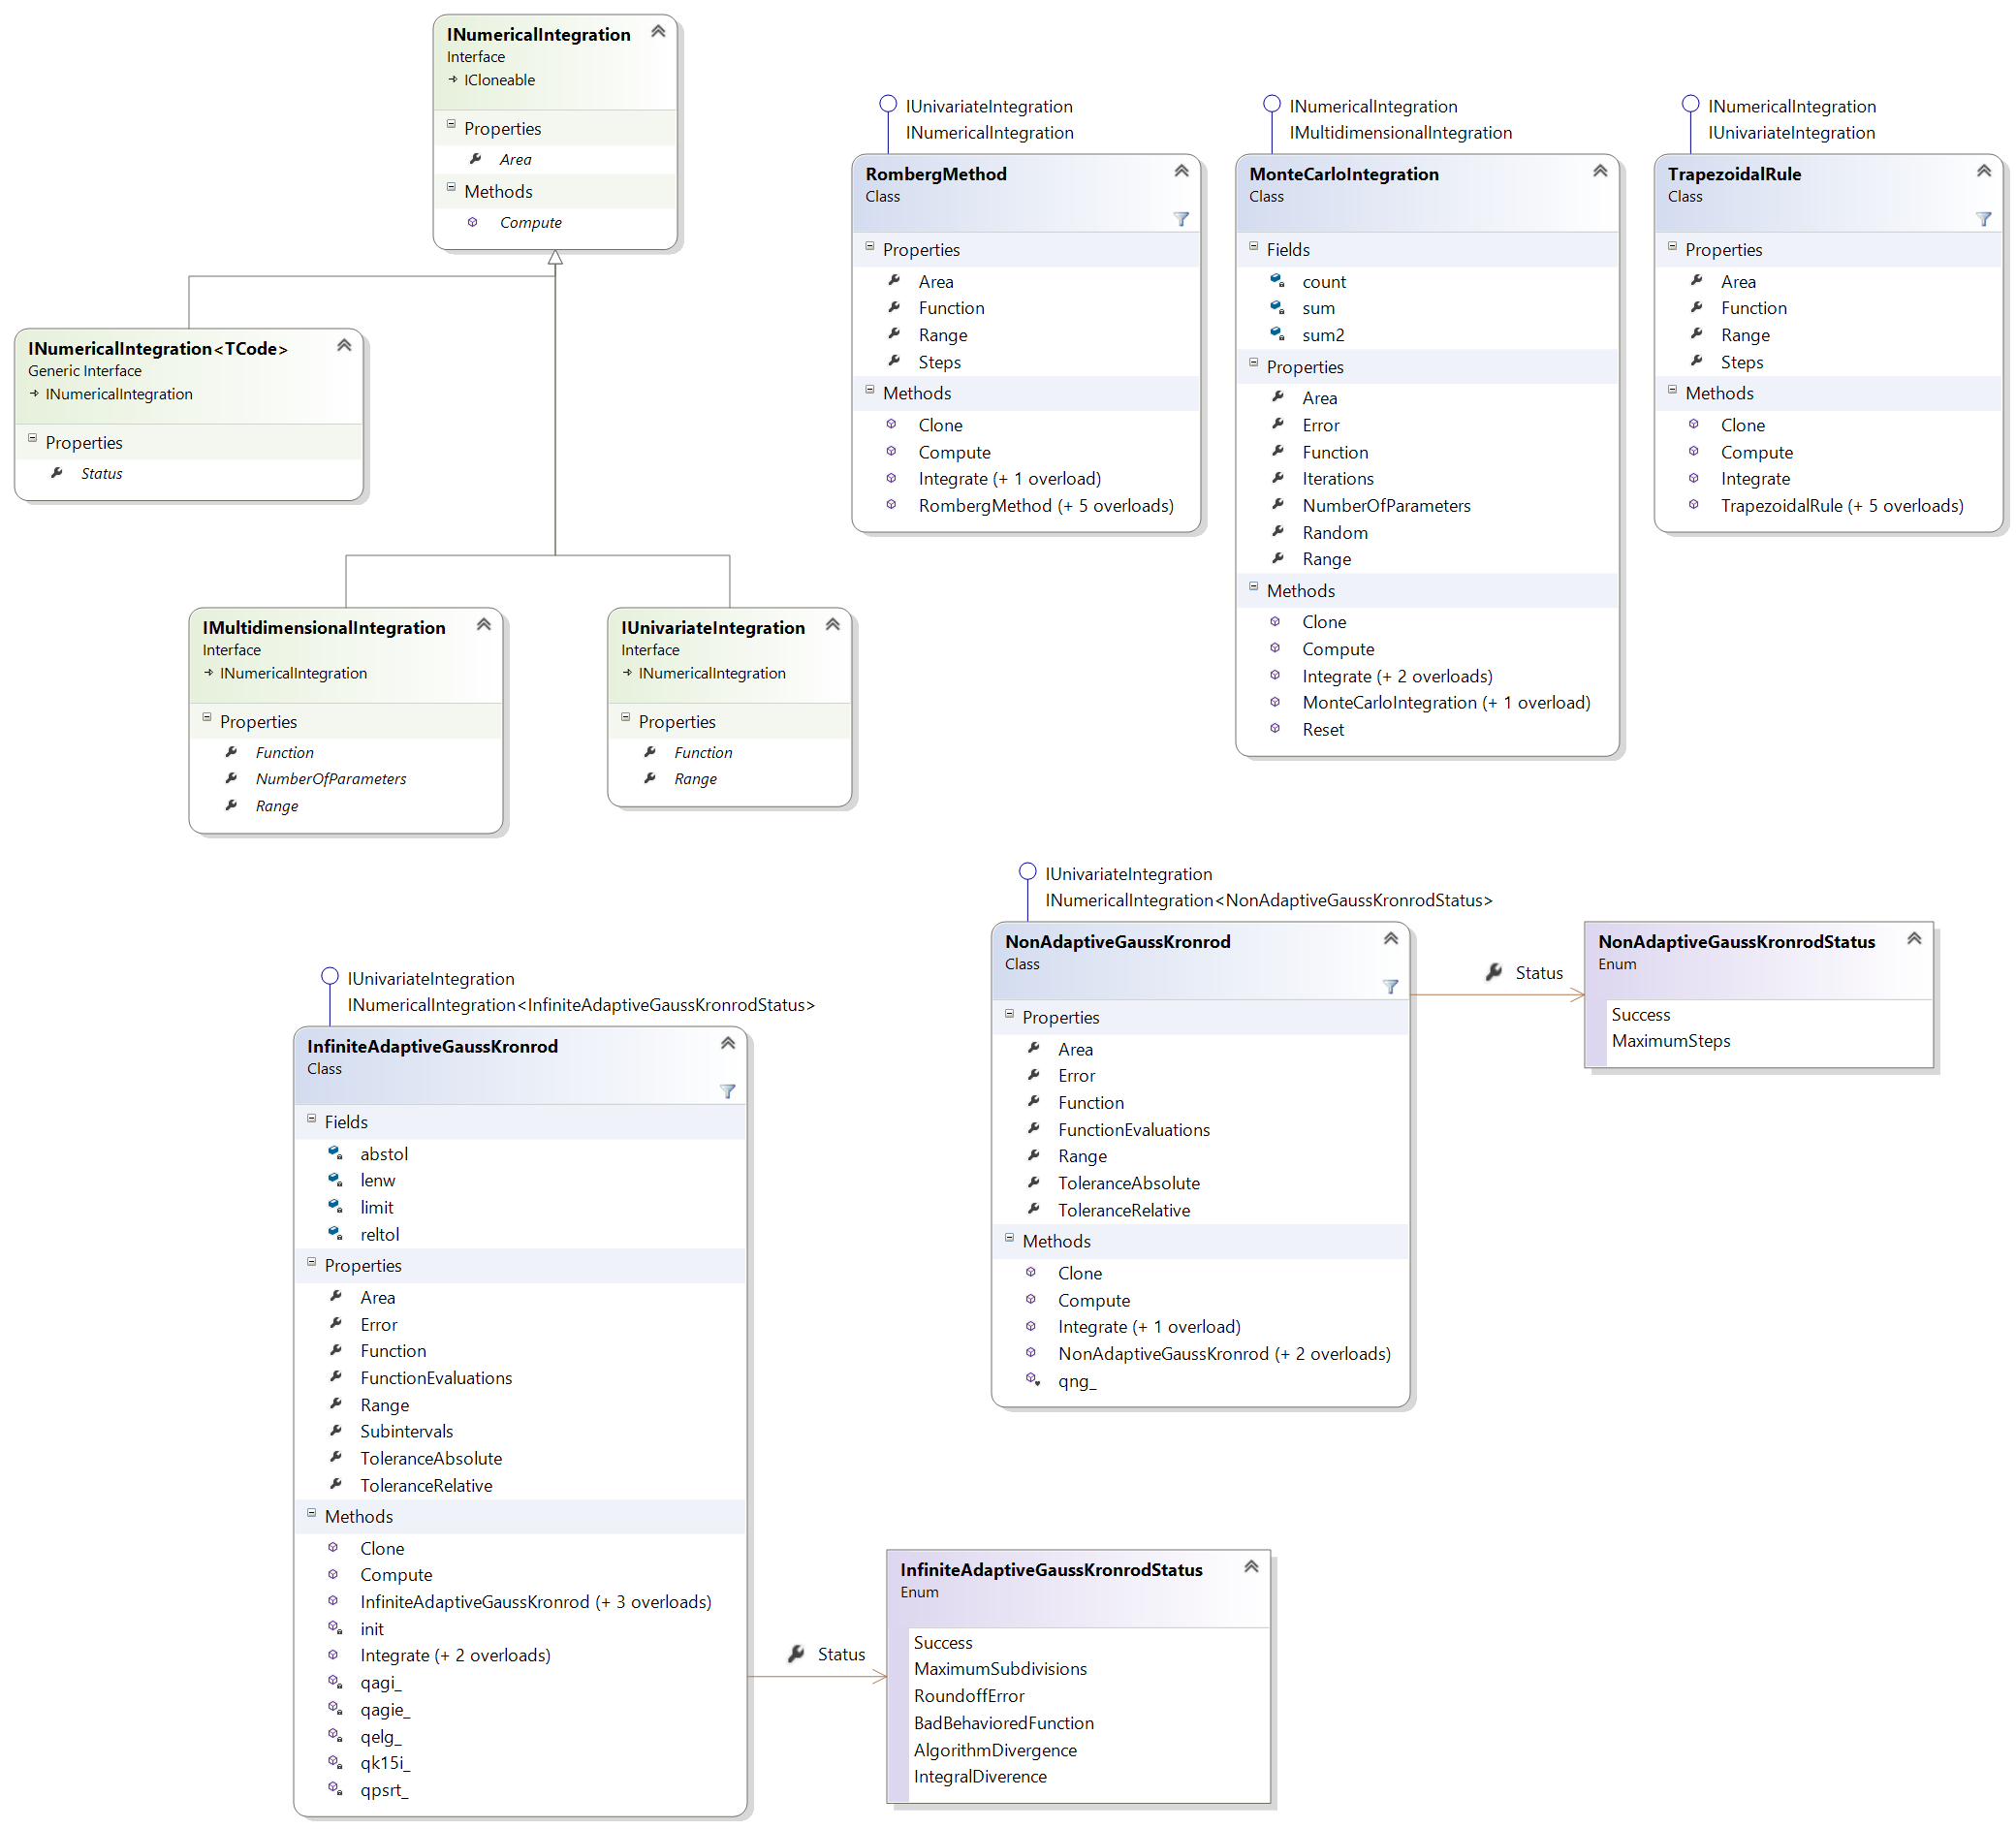
\includegraphics{Pictures/Accord.Math.Integration.png}
\caption{Accord.Math.Integration Classes Provided under the Creative
Commons Attribution/Share-Alike License}
\end{figure}

The \texttt{Accord.Neuro} is useful for any neural network structures.
The visualization features of Accord can be used during testing,
benchmarking, and development of our implementation to better show our
progress and metrics \autocite{accord}.

Accord is made available in the NuGet package manager, making it easily
integrated into our Visual Studio project environment.

\subsubsection{Input from Unity
Interface}\label{input-from-unity-interface}

Using the \texttt{putImage} method in the primary \texttt{CVInterface}
class we will be importing images captured by the Intel® RealSense™
camera after it is passed through the Unity interface. These images will
be read in and stored using the \texttt{System.Drawing.Bitmap} format.
This format's pixel structure can be altered depending on the needs of
the computer vision implementation.

\subsubsection{Random Forest
Implementation}\label{random-forest-implementation}

Our implementation of the auto-context random forest suggested in
``Uncertainty-Driven 6D Pose Estimation of Objects and Scenes from a
Single RGB Image'' will be built using the
\texttt{Accord.MachineLearning} namespace. More specifically the
structure will be built with the \texttt{RandomForest},
\texttt{DecisionTree}, and \texttt{DecisionNode} classes. The random
forest will first use the built-in learning functions for training and
later be modified to more closely resemble the training of Brachmann
\emph{et al.} \autocites{brachmann}{accord}.

\subsubsection{RANSAC Implementation}\label{ransac-implementation}

Our random sampling consensus (RANSAC) implementation will be built to
approximately mimic the implementation explained in ``Uncertainty-Driven
6D Pose Estimation of Objects and Scenes from a Single RGB Image''
\autocite{brachmann}. The \texttt{RANSAC\textless{}TModel\textgreater{}}
class in the Accord.NET framework will be utilized to create our
implementation \autocite{accord}. This implementation will be modified
to run parallel hypothesis checks to follow the structure of preemptive
RANSAC.

Our instance of RANSAC will have a set of Hypotheses which have the pose
information stored. During processing these will be culled, refined, and
added to as necessary.

\subsubsection{Pose Refinement
Implementation}\label{pose-refinement-implementation}

We would like to implement a similar method to Brachmann \emph{et al.}
to refine the poses gathered by RANSAC \autocite{brachmann}. Each
Hypothesis in the RANSAC instance will have a refinement method called
\texttt{refine()} which will be able to improve the pose estimation if
that hypothesis is chosen for refinement. The poses chosen for
refinement will be handled within our RANSAC implementation.

\subsubsection{Output to the Unity
Interface}\label{output-to-the-unity-interface}

The metadata associated with each detected object will be exported to
Unity in a data-structure containing the x translation, y translation, z
translation, x rotation, y rotation, z rotation, scale, and the object
type according to the pre-existing 3D models. The translation values
will provided according to the estimated center of the observed scene.
This information will then be used to create and transform the object in
a Unity scene.

\subsection{Unity Design}\label{unity-design}

When the user starts up Unity, they will be directed to the base Unity
Editor screen which is shown right under. From there, they will have the
option to go into the Window tab and select our custom screen.

\begin{figure}
\centering
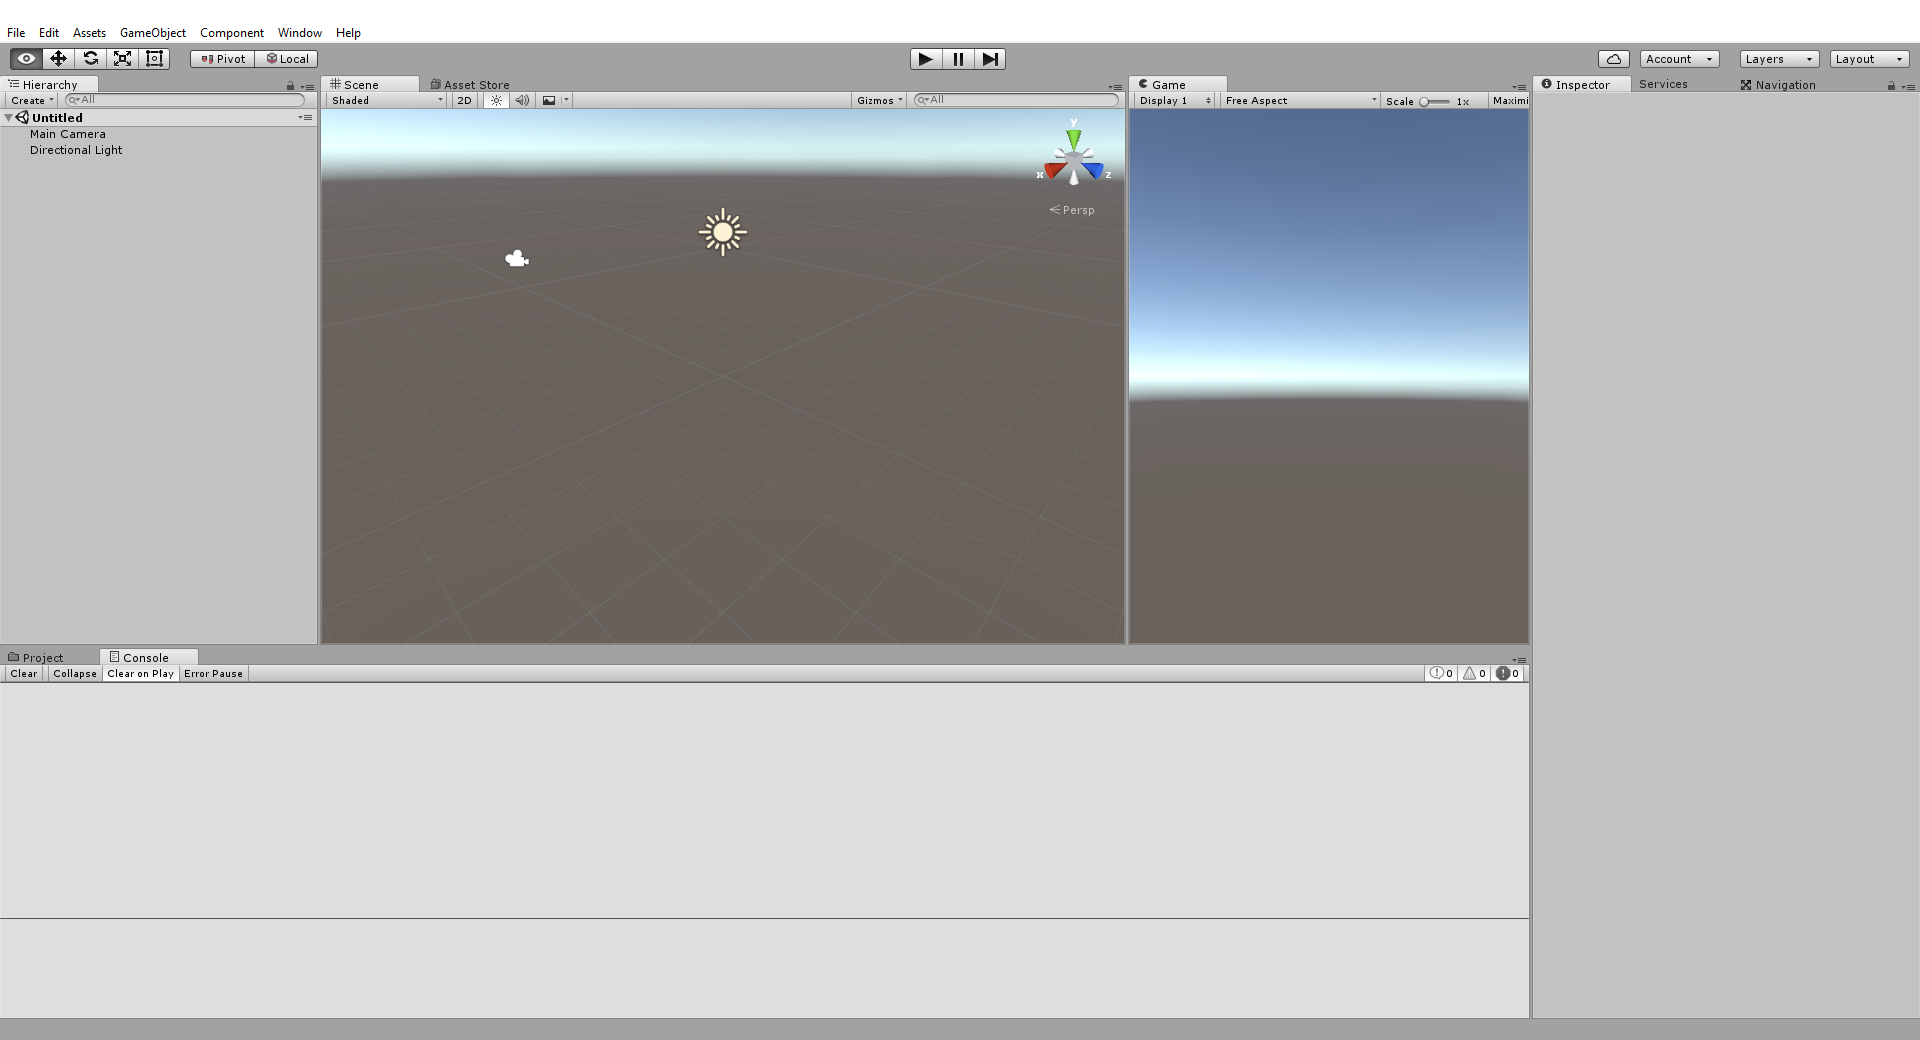
\includegraphics{Pictures/UnityHomeScreen.png}
\caption{Unity Editor Home Screen}
\end{figure}

\subsubsection{Custom Window}\label{custom-window}

The design of the Unity module will be centered around 2 different
parts. The first part is the UI/central control class which will
implement and create a new Unity Editor window. This window will contain
the button that the user can press to begin the plugins function. On
initial press of the button, the UI will call on the camera module's
interface. It will wait for the camera to send images back, which it
will then feed to the computer vision interface so that the computer
vision module can process the images. An example of a simple custom
screen and the script in the assets is shown below, without any of the
functionality described above.

\begin{figure}
\centering
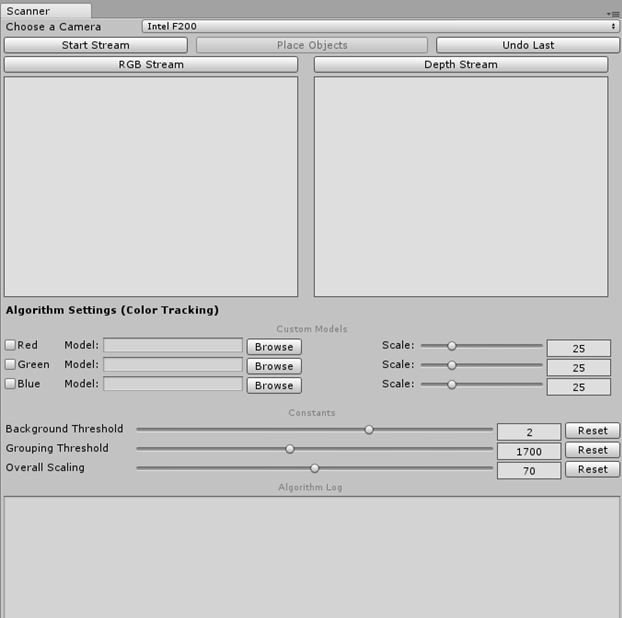
\includegraphics{Pictures/editorwindow.png}
\caption{Unity Test Custom Window}
\end{figure}

\paragraph{UI Features}\label{ui-features}

While the plugin is in different stages of execution, the overall status
will be translated into user-friendly terms, outputted as a string, and
displayed as a label in the window. When the camera starts up, the label
will display ``Scanning Objects\ldots{}'' and will continue displaying
that label until the camera software stops sending images back to the
UI/Controller class. Once the images stop, the label will switch to
``Processing Images\ldots{}'' while the computer vision module processes
the scanned images into a usable format for the Object Creator. The time
that it takes the Object Creator to spawn the items on the scene should
be negligible enough such that a label is not needed, but should the
time be noticeable, the label may be switched to ``Drawing Scanned
Objects'' while the Object Creator executes it's task. Once the plugin's
execution is finished, the UI/Controller will revert back to a ready
state to potentially scan one more time.

\paragraph{Objects to Draw}\label{objects-to-draw}

The processed images will return in the form of a list comprised of
type, translation, rotation, and scale. The type refers to the types of
the the specific objects scanned. Our implementation will call for
prebuilt assets to be stored in our plugin files as prefabs that are
base versions of all possible blocks that will be scanned into the Unity
project. Should more block shapes be introduced into the algorithm, our
sponsors have already agreed to create base models for us to use in
Unity. The prebuilt objects that we already have at our disposal are:

\begin{itemize}
\tightlist
\item
  cubes
\item
  cones
\item
  cylinders
\item
  rectangular prisms
\item
  pyramids
\item
  bridges
\item
  wedges/ramps
\end{itemize}

The Translation refers to the position of the objects with respect to
the origin of the world space in the Unity Scene. This attribute will
determine exactly where the model is rendered in the scene. The current
plan is to have a reference measurement which can be converted into
Unity World Space coordinates.

The Rotation refers to the degrees around the object's 3 center axes (x,
y, z) that the object is moving circularly. The rotation can go from 0
degrees up to 360 degrees (360 being the original starting position).
Unity allows users to change an object's rotation through using Euler
Angles and the rotations themselves are stored in Unity as Quaternions.

The Scale refers to the size of the object with respect to the original
object that it is modelled off of. For example, a cube that is twice as
wide, long, and high as the normal cube used will have a scale of 2 in
all directions. Having this implementation will allow for multiple block
types to be used without having to restrict the user to a specific brand
of blocks. The original block's scale will be saved and compared to the
scanned blocks, allowing the Unity module to scale the stored prefab to
whatever it needs to be.

\subsubsection{Object Creator}\label{object-creator}

The object creator is the class that the UI class will feed the
processed object data to. This class extends Unity's MonoBehavior and is
what makes the calls to draw the objects onto the scene. Unity has a
method called \texttt{Instantiate()} that allows one to instantiate
prefabs through a script. The Instantiate method has multiple
constructors that can be called to load a prefab. The one that will be
mainly used in this class is:

\texttt{public\ static\ Object\ Instantiate(Object\ original,\ Vector3\ position,\ Quaternion\ rotation);}

This instantiation will allow us to set a variable equal to the newly
instantiated prefab that is already set to the position and rotation
necessary. From there the variable can be used to adjust the scale
attribute for the newly created GameObject.

\section{Design Summary}\label{design-summary}

\subsection{Camera Module UML}\label{camera-module-uml}

The final overall design of the camera module is displayed below. This
includes the organization of the classes used as well as the flow of
activities.

\subsubsection{Camera Module Class
Diagram}\label{camera-module-class-diagram}

The following is the design of the Camera module. All access to the
camera module is handled through the ICamera interface. This allows the
commands called by the Unity Module to stay constant while the
implementation of the Camera Module is free to change. The

\begin{figure}
\centering
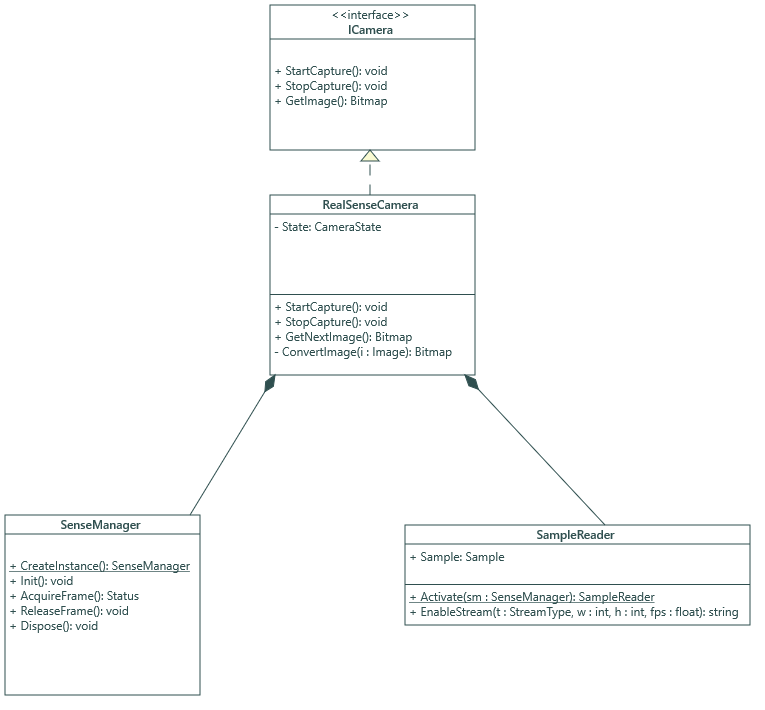
\includegraphics{Figures/CameraModuleClass.png}
\caption{Camera Module Class Diagram}
\end{figure}

\subsubsection{Camera Module Activity
Diagram}\label{camera-module-activity-diagram}

The following is the flow of activity within the class diagram. Once
start has been called, the Intel® RealSense™ pipeline is initiated and
will continually capture data frames until the caller has called stop.
These captured frames are available via the \texttt{GetImage} method of
the \texttt{ICamera} interface.

\begin{figure}
\centering
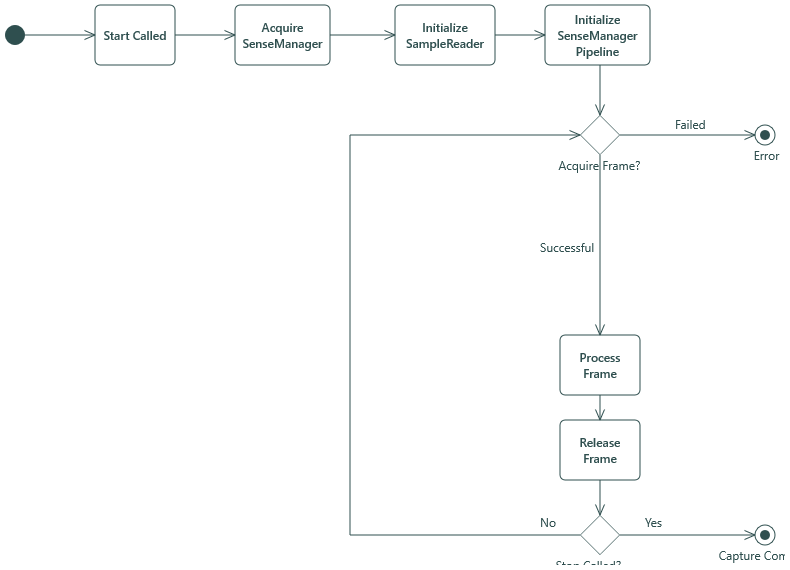
\includegraphics{Figures/CameraModuleActivity.png}
\caption{Camera Module Activity Diagram}
\end{figure}

\subsection{Computer Vision UML}\label{computer-vision-uml}

The following UML diagram gives a general overview of the planned
computer vision implementation for this project. The more fine-grained
details such as parameters, methods, and types are still subject to
change as development continues, but the general structure and ideas
will remain the same.

\begin{figure}
\centering
\includegraphics{Figures/CV_class.png}
\caption{Computer Vision Class Diagram}
\end{figure}

\subsection{Unity UML}\label{unity-uml}

The following Activity Diagram gives a general high-level description of
how the Unity module will work when called.

\begin{figure}
\centering
\includegraphics{Figures/unityActivityDiagram.png}
\caption{Unity Activity Diagram}
\end{figure}

\subsection{Overview UML}\label{overview-uml}

\section{Development Environment and
Operations}\label{development-environment-and-operations}

\subsection{IDE}\label{ide}

We are using Microsoft Visual Studio 2015 Community Edition in order to
develop our project. We chose Microsoft Visual Studio 2015 Community
Edition because, it offers support for Unity Plugin development as well
as excellent support for C\# development. All the members on our team
also have substantial experience with the IDE. Microsoft Visual Studio
also helps to simplify the build process for multiple dependent
projects. Visual Studio also features the NuGet Package Manager which is
an incredibly helpful tool for adding libraries, frameworks, or
dependencies to a project. The Accord.NET framework is available as a
NuGet package and can be easily integrated with the Visual Studio
environment. Finally Microsoft Visual Studio also has excellent
integration with the Git version control system which will help
facilitate rapid development by multiple authors on our team.

\subsection{Version Control System}\label{version-control-system}

We chose to use Git as our version control system. We decided on Git due
to our group members' familiarity with the system as well as its cost.
All of our team members have worked with Git in the past, therefore we
were able to incorporate the tool into our developer operations without
any further training needed. Also since Git is free, it will not carry a
cost to our sponsors or our team members. We are hosting our Git
repository on GitHub. Hosting on GitHub is also free for public
repositories, which we are able to use since we are not subject to an
nondisclosure agreement. In addition to repository hosting, GitHub also
offers some valuable tools to assist in developer coordination. We are
making use of the issue tracking system within GitHub in order to
coordinate the status of various features and bug fixes.

\subsection{Documentation}\label{documentation}

In order to safely document our project using multiple authors, we
needed to incorporate version-control-compatible formatting into this
documentation's development environment. We used the Markdown mark up
language in combination with Pandoc to facilitate our authoring and
presentation of our documentation content.

\subsubsection{Markdown}\label{markdown}

We are using Markdown for documenting purposes. Markdown is a simple
plaintext format with allows for writing documents with common features
such as: headers, lists, and tables. We chose to use Markdown because it
is easy to version control as well as being a widespread format. Because
Markdown is a plaintext format, multiple group members can work on it at
the same time and Git is able to easily merge their changes. This is in
contrast to a binary format such as *.docx whose line changes Git cannot
merge. Also since Markdown has become such a widespread format there is
plenty of tooling to support its authoring and conversion. We chose
Markdown over similar formats such as LaTex and HTML because its syntax
is much simpler. This makes Markdown easy to learn as well as quick to
write. Without Markdown, our documentation process would be slower and
more prone to data loss.

\subsubsection{Pandoc}\label{pandoc}

We used to Pandoc to convert our Markdown to more presentation oriented
formats. This tool allows us to easily develop, merge, and version
control our documentation while also being able to support visually
appealing presentation file formats such as \emph{.docx and }.pdf.
Without Pandoc we would be forced to use binary formats which would make
it difficult to version control our documentation.

\section{Testing Plan}\label{testing-plan}

\subsection{CameraModule Testing}\label{cameramodule-testing}

The primary aspects of the camera module that need to be tested are: the
public interface and the image conversion capabilities.

\subsubsection{Unit Tests}\label{unit-tests}

The unit tests will be used to test the behavior of each function
individually in different circumstances. The parameters of each test are
as follows:

\begin{itemize}
\tightlist
\item
  \textbf{Input} - The explicit parameters passed into each function.
  The value ``N/A'' will be used if the function takes no parameters.
\item
  \textbf{Output} - The value which the function returns. The value
  ``N/A'' will be used if the function is void
\item
  \textbf{Starting Conditions} - Any significant state values that
  should be set before the start of the test. The value ``N/A'' will be
  used if there are not any consequential initial state values.
\item
  \textbf{Ending Conditions} - Any significant state values that should
  be present as a result of the method being tested. The value ``N/A''
  will be used if there are not any consequential state values.
\end{itemize}

\paragraph{StartCapture}\label{startcapture-1}

The job of the \texttt{StartCapture} method is to signal to the rest of
the \texttt{RealSenseCamera} that capture should begin. This starts the
capture loop and updates the \texttt{State} member to
\texttt{CameraState.RUNNING}.

\begin{longtable}[]{@{}llll@{}}
\toprule
Input & Output & Starting Conditions & Ending Conditions\tabularnewline
\midrule
\endhead
N/A & N/A & State == CameraState.STOPPED & State ==
CameraState.RUNNING\tabularnewline
\bottomrule
\end{longtable}

\paragraph{StopCapture}\label{stopcapture-1}

The job of the \texttt{StopCapture} method is simply to signal to the
rest of the \texttt{RealSenseCamera} class that the capture should halt.
This is used to signal to the capture loop to terminate execution.

\begin{longtable}[]{@{}llll@{}}
\toprule
Input & Output & Starting Conditions & Ending Conditions\tabularnewline
\midrule
\endhead
N/A & N/A & State == CameraState.RUNNING & State ==
CameraState.STOPPED\tabularnewline
\bottomrule
\end{longtable}

\paragraph{ConvertImage}\label{convertimage}

The only way to objectively test the \texttt{ConvertImage} method is to
procedurally generate \texttt{Image} objects from the Intel® RealSense™
SDK as input for the \texttt{ConvertImage} method. A brief description
of the attributes are below:

\begin{itemize}
\tightlist
\item
  \textbf{TestRSImage1} - All pixels are set to black
\item
  \textbf{TestRSImage2} - Simple white background with black text in the
  foreground
\item
  \textbf{TestRSImage3} - Picture of the table with blocks
\end{itemize}

The test would make sure that the \texttt{Bitmap} (denoted as
ImageGeneratingBitmap\#) that was used to produce the Intel® RealSense™
SDK \texttt{Image} objects (denoted as TestRSImage\#) are what the
\texttt{ConvertImage} method produces.

\begin{longtable}[]{@{}llll@{}}
\toprule
Input & Output & Starting Conditions & Ending Conditions\tabularnewline
\midrule
\endhead
TestRSImage1 & ImageGeneratingBitmap1 & N/A & N/A\tabularnewline
TestRSImage2 & ImageGeneratingBitmap2 & N/A & N/A\tabularnewline
TestRSImage3 & ImageGeneratingBitmap3 & N/A & N/A\tabularnewline
\bottomrule
\end{longtable}

\subsection{Computer Vision Testing}\label{computer-vision-testing}

\subsubsection{Benchmark Testing}\label{benchmark-testing}

We will be using the CVPR 2016 code included with ``Uncertainty-Driven
6D Pose Estimation of Objects and Scenes from a Single RGB Image'' as a
benchmark for our computer vision interface. We would like to track
metrics on our training and detection processes to attempt to get as
close as possible to the results of Bachmann \emph{et al.}.

On the Hinterstoisser dataset Bachmann \emph{et al.} achieved 82.1\%
accuracy when estimating 3D 6-DOF pose with a maximum re-projection
error for all vertices of 5cm and a maximum rotation error of 5°.
Processing time was calculated at a maximum of 1 second for 13 objects,
nearly 2 seconds for 25 objects and nearly 4 seconds for 50 images
{[}{]}. The issue with utilizing processing time is that the authors
mention that processing time can broadly vary with hypothesis
acceptance. If it is more difficult to accept a hypothesis, the
processing time increases. We will mitigate this risk by testing both
their implementation and our implementation on the same data after being
trained on the same dataset and compare those recorded processing times.
Their processing times and prediction-recall graph are pictured below in
figure 5 from {[}{]}.

\begin{figure}
\centering
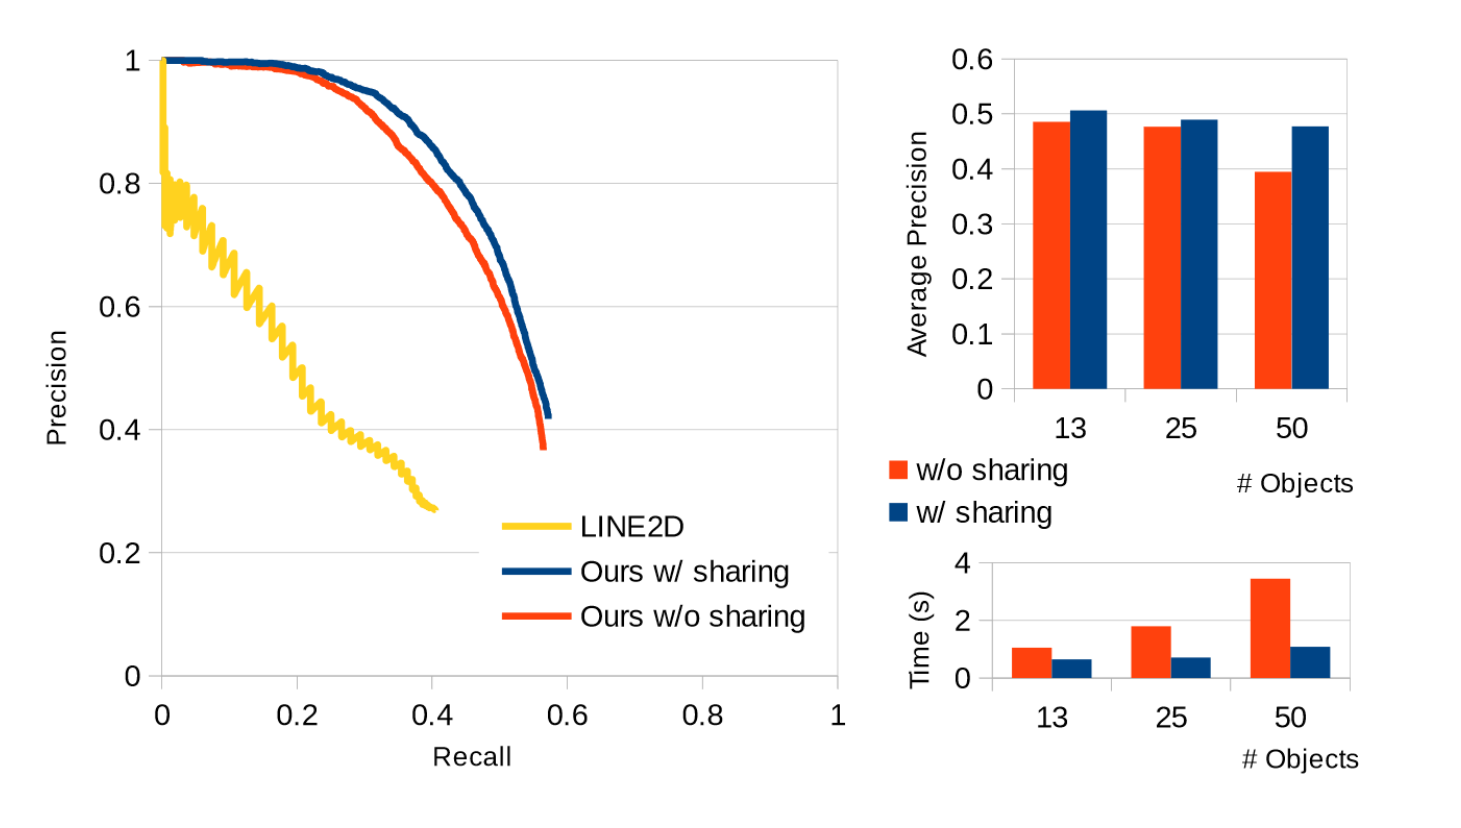
\includegraphics{Pictures/figure5.png}
\caption{Experiment Results from Brachmann \emph{et al.}}
\end{figure}

The primary classes for benchmark testing in the CVPR 2016
implementation of ``Uncertainty-Driven 6D Pose Estimation of Objects and
Scenes from a Single RGB Image'' are \texttt{train\_trees} and
\texttt{test\_pose\_estimation}. \texttt{train\_trees} monitors training
time by using the \texttt{stopWatch} function for accurate time tracking
and in \texttt{test\_pose\_estimation} the average RANSAC runtime, the
average auto-context random forest runtime, and the evaluation results
are given in \texttt{avgRansacTime},\texttt{avgForestTime}, and
\texttt{objEval} respectively. We will use these recorded measures on
different datasets, beginning with the Hinerstoisser dataset, as targets
for our implementation running on the same datasets.

\subsubsection{Accord Framework Unit
Tests}\label{accord-framework-unit-tests}

The Accord.NET framework includes some unit tests for each major
namespace to allow the user to verify the integrity of the framework. We
will run the unit tests for each namespace we will be utilizing to
ensure that they are functioning as expected \autocite{accord}.

\begin{longtable}[]{@{}ll@{}}
\toprule
Test & Namespace\tabularnewline
\midrule
\endhead
Validate full namespace & Accord.Tests.MachineLearning\tabularnewline
Test Decision Tree & Accord.Tests.MachineLearning\tabularnewline
Test Decision Tree Rules & Accord.Tests.MachineLearning\tabularnewline
Test Random Forest & Accord.Tests.MachineLearning\tabularnewline
Test Decision Tree C45 Learning &
Accord.Tests.MachineLearning\tabularnewline
Test RANSAC & Accord.Tests.MachineLearning\tabularnewline
Test Matrix Math & Accord.Tests.Math\tabularnewline
Test Point3 & Accord.Tests.Math\tabularnewline
Test Integrals & Accord.Tests.Math\tabularnewline
Test Monte Carlo Integration & Accord.Tests.Math\tabularnewline
\bottomrule
\end{longtable}

\subsubsection{Unit Testing}\label{unit-testing}

The first set of computer vision tests will begin in late December 2016
and continue through early January 2017. These tests will consist of
integrity verification of the Accord.NET framework. We will ensure that
the framework is performing as expected and the desired data-structures
are built, modified, and run as efficiently as the team expects. Sample
code included with the framework will be compiled and run for each of
the major features to be implemented in the computer vision interface of
our project.

\paragraph{RANSAC Tests}\label{ransac-tests}

\begin{longtable}[]{@{}lll@{}}
\toprule
\begin{minipage}[b]{0.06\columnwidth}\raggedright\strut
Date\strut
\end{minipage} & \begin{minipage}[b]{0.16\columnwidth}\raggedright\strut
Test Purpose\strut
\end{minipage} & \begin{minipage}[b]{0.22\columnwidth}\raggedright\strut
Expected Outcome\strut
\end{minipage}\tabularnewline
\midrule
\endhead
\begin{minipage}[t]{0.06\columnwidth}\raggedright\strut
Dec. 2016 - Jan. 2017\strut
\end{minipage} & \begin{minipage}[t]{0.16\columnwidth}\raggedright\strut
Verify Accord RANSAC\strut
\end{minipage} & \begin{minipage}[t]{0.22\columnwidth}\raggedright\strut
Sample code runs and performs as advertised.\strut
\end{minipage}\tabularnewline
\begin{minipage}[t]{0.06\columnwidth}\raggedright\strut
Feb. 2017\strut
\end{minipage} & \begin{minipage}[t]{0.16\columnwidth}\raggedright\strut
Basic RANSAC Function Test\strut
\end{minipage} & \begin{minipage}[t]{0.22\columnwidth}\raggedright\strut
RANSAC can be run on placeholder data with appropriate results.\strut
\end{minipage}\tabularnewline
\begin{minipage}[t]{0.06\columnwidth}\raggedright\strut
Mar. 2017\strut
\end{minipage} & \begin{minipage}[t]{0.16\columnwidth}\raggedright\strut
Fully Functioning RANSAC\strut
\end{minipage} & \begin{minipage}[t]{0.22\columnwidth}\raggedright\strut
RANSAC runs on real data gathered from the Random Forest.\strut
\end{minipage}\tabularnewline
\begin{minipage}[t]{0.06\columnwidth}\raggedright\strut
Apr. 2017\strut
\end{minipage} & \begin{minipage}[t]{0.16\columnwidth}\raggedright\strut
RANSAC Performance Benchmarking\strut
\end{minipage} & \begin{minipage}[t]{0.22\columnwidth}\raggedright\strut
RANSAC runs with comparable measurements to stat-of-the-art
methods.\strut
\end{minipage}\tabularnewline
\bottomrule
\end{longtable}

\paragraph{Random Forest Tests}\label{random-forest-tests}

\begin{longtable}[]{@{}lll@{}}
\toprule
\begin{minipage}[b]{0.06\columnwidth}\raggedright\strut
Date\strut
\end{minipage} & \begin{minipage}[b]{0.16\columnwidth}\raggedright\strut
Test Purpose\strut
\end{minipage} & \begin{minipage}[b]{0.22\columnwidth}\raggedright\strut
Expected Outcome\strut
\end{minipage}\tabularnewline
\midrule
\endhead
\begin{minipage}[t]{0.06\columnwidth}\raggedright\strut
Dec. 2016 - Jan. 2017\strut
\end{minipage} & \begin{minipage}[t]{0.16\columnwidth}\raggedright\strut
Verify Accord Random Forests\strut
\end{minipage} & \begin{minipage}[t]{0.22\columnwidth}\raggedright\strut
Sample code runs and performs as advertised.\strut
\end{minipage}\tabularnewline
\begin{minipage}[t]{0.06\columnwidth}\raggedright\strut
Feb. 2017\strut
\end{minipage} & \begin{minipage}[t]{0.16\columnwidth}\raggedright\strut
Random Forest Training Test\strut
\end{minipage} & \begin{minipage}[t]{0.22\columnwidth}\raggedright\strut
Ensure RFs can be trained using built-in \texttt{Learn()} method.\strut
\end{minipage}\tabularnewline
\begin{minipage}[t]{0.06\columnwidth}\raggedright\strut
Mar. 2017\strut
\end{minipage} & \begin{minipage}[t]{0.16\columnwidth}\raggedright\strut
Random Forest Testing\strut
\end{minipage} & \begin{minipage}[t]{0.22\columnwidth}\raggedright\strut
Forest is trained and can be used for predictions on image input with
appropriate leaf values.\strut
\end{minipage}\tabularnewline
\begin{minipage}[t]{0.06\columnwidth}\raggedright\strut
Apr. 2017\strut
\end{minipage} & \begin{minipage}[t]{0.16\columnwidth}\raggedright\strut
Random Forest Performance Benchmarking\strut
\end{minipage} & \begin{minipage}[t]{0.22\columnwidth}\raggedright\strut
Forest should be used for object predictions in reasonable time and with
sufficiently accurate leaf values when compared to state-of-the-art
methods.\strut
\end{minipage}\tabularnewline
\bottomrule
\end{longtable}

\paragraph{Input Tests}\label{input-tests}

\begin{longtable}[]{@{}lll@{}}
\toprule
\begin{minipage}[b]{0.06\columnwidth}\raggedright\strut
Date\strut
\end{minipage} & \begin{minipage}[b]{0.16\columnwidth}\raggedright\strut
Test Purpose\strut
\end{minipage} & \begin{minipage}[b]{0.22\columnwidth}\raggedright\strut
Expected Outcome\strut
\end{minipage}\tabularnewline
\midrule
\endhead
\begin{minipage}[t]{0.06\columnwidth}\raggedright\strut
Jan. 2017\strut
\end{minipage} & \begin{minipage}[t]{0.16\columnwidth}\raggedright\strut
Get an Image\strut
\end{minipage} & \begin{minipage}[t]{0.22\columnwidth}\raggedright\strut
Receive an image from the camera interface in the correct format.\strut
\end{minipage}\tabularnewline
\begin{minipage}[t]{0.06\columnwidth}\raggedright\strut
Feb. 2017\strut
\end{minipage} & \begin{minipage}[t]{0.16\columnwidth}\raggedright\strut
Get a Series of Images\strut
\end{minipage} & \begin{minipage}[t]{0.22\columnwidth}\raggedright\strut
Receive multiple images at an appropriate rate according to processing
time estimates.\strut
\end{minipage}\tabularnewline
\begin{minipage}[t]{0.06\columnwidth}\raggedright\strut
Mar. 2017\strut
\end{minipage} & \begin{minipage}[t]{0.16\columnwidth}\raggedright\strut
Camera Angle Tests\strut
\end{minipage} & \begin{minipage}[t]{0.22\columnwidth}\raggedright\strut
Ensure the optimal camera setup for pitch and distance to receive the
best results from the algorithm.\strut
\end{minipage}\tabularnewline
\bottomrule
\end{longtable}

\paragraph{Output Tests}\label{output-tests}

\begin{longtable}[]{@{}lll@{}}
\toprule
\begin{minipage}[b]{0.06\columnwidth}\raggedright\strut
Date\strut
\end{minipage} & \begin{minipage}[b]{0.16\columnwidth}\raggedright\strut
Test Purpose\strut
\end{minipage} & \begin{minipage}[b]{0.22\columnwidth}\raggedright\strut
Expected Outcome\strut
\end{minipage}\tabularnewline
\midrule
\endhead
\begin{minipage}[t]{0.06\columnwidth}\raggedright\strut
Jan. 2017\strut
\end{minipage} & \begin{minipage}[t]{0.16\columnwidth}\raggedright\strut
Output a Structure\strut
\end{minipage} & \begin{minipage}[t]{0.22\columnwidth}\raggedright\strut
Output a data-structure to Unity holding placeholder data.\strut
\end{minipage}\tabularnewline
\begin{minipage}[t]{0.06\columnwidth}\raggedright\strut
Mar. 2017\strut
\end{minipage} & \begin{minipage}[t]{0.16\columnwidth}\raggedright\strut
Output Real Data\strut
\end{minipage} & \begin{minipage}[t]{0.22\columnwidth}\raggedright\strut
Output pose information gathered in RANSAC into the Unity
interface.\strut
\end{minipage}\tabularnewline
\bottomrule
\end{longtable}

\subsection{Unity Testing}\label{unity-testing}

\begin{longtable}[]{@{}lll@{}}
\toprule
\begin{minipage}[b]{0.06\columnwidth}\raggedright\strut
Date\strut
\end{minipage} & \begin{minipage}[b]{0.16\columnwidth}\raggedright\strut
Test Purpose\strut
\end{minipage} & \begin{minipage}[b]{0.22\columnwidth}\raggedright\strut
Expected Outcome\strut
\end{minipage}\tabularnewline
\midrule
\endhead
\begin{minipage}[t]{0.06\columnwidth}\raggedright\strut
Jan. 2017\strut
\end{minipage} & \begin{minipage}[t]{0.16\columnwidth}\raggedright\strut
UI Button and Label Tests\strut
\end{minipage} & \begin{minipage}[t]{0.22\columnwidth}\raggedright\strut
Change labels and button text as the UI state changes.\strut
\end{minipage}\tabularnewline
\begin{minipage}[t]{0.06\columnwidth}\raggedright\strut
Jan. 2017\strut
\end{minipage} & \begin{minipage}[t]{0.16\columnwidth}\raggedright\strut
Camera Output\strut
\end{minipage} & \begin{minipage}[t]{0.22\columnwidth}\raggedright\strut
Test main UI class calls to camera and that it receives camera output
correctly.\strut
\end{minipage}\tabularnewline
\begin{minipage}[t]{0.06\columnwidth}\raggedright\strut
Feb. 2017\strut
\end{minipage} & \begin{minipage}[t]{0.16\columnwidth}\raggedright\strut
Object Creation\strut
\end{minipage} & \begin{minipage}[t]{0.22\columnwidth}\raggedright\strut
Instantiate object prefabs with mock input and have them show up on
screen.\strut
\end{minipage}\tabularnewline
\begin{minipage}[t]{0.06\columnwidth}\raggedright\strut
Mar.. 2017\strut
\end{minipage} & \begin{minipage}[t]{0.16\columnwidth}\raggedright\strut
CV Data Tests\strut
\end{minipage} & \begin{minipage}[t]{0.22\columnwidth}\raggedright\strut
Test Object Creator with data output from cv module.\strut
\end{minipage}\tabularnewline
\bottomrule
\end{longtable}

\subsection{Integration Testing}\label{integration-testing}

As mentioned in the above test cases, by January 2017, when we have
access to the necessary hardware for testing, the camera interface will
be able to output an image in a bitmap format to the Unity interface.
The Unity interface will then receive the input image data from the
camera interface and send it to the computer vision interface. The
computer vision interface will then output placeholder information into
the Unity interface, completing the flow of data in our application.
This will allow us to begin integration tests.

\section{Budget and Resources Provided by
Sponsors}\label{budget-and-resources-provided-by-sponsors}

Our sponsors did not specify a specific dollar amount for our budget but
our possible costs are highly controlled. The UCF Games Research Group
has many resources available for our team to utilize for this project.
All possible costs or necessary resources are described below.

\subsection{Cameras}\label{cameras}

The Intel® RealSense™ F200 was already available to the UCF Games
Research Group. Therefore the use of the camera will not carry a cost to
our group. The only potential cost the camera could pose is if we find
the Intel® RealSense™ F200 camera to be unusable and we have to use a
camera that the UCF Games Research Group does not already have in their
possession. They also have a Microsoft Kinect, Microsoft Hololens, and
an HTC Vive.

\subsection{Working Area}\label{working-area}

The UCF Games Research Group has an office space with computers,
cameras, and space for team collaboration. This area provides ample
space for our team to work with the cameras and a table with objects
placed on it.

\subsection{Expert Consultation}\label{expert-consultation}

Under the UCF Games Research group, we have contact with students and
experts in various fields that can be useful for help with the
development process. We have access to the following:

\begin{itemize}
\item
  Unity experts to consult in order to learn and work with the
  intricacies of the Unity Software.
\item
  3D models to create assets that may be required for the process of
  instantiating the models within the Unity Platform
\end{itemize}

\section{Challenges}\label{challenges}

\subsection{Computer Vision Algorithmic
Complexities}\label{computer-vision-algorithmic-complexities}

The Computer Vision problem that our team is working through is still
part of a very active field of research. With this in mind, the members
of our team who will be focusing on the Computer Vision interface will
need to at least partially catch up to this active field in order to
successfully implement a useful algorithm. Our team will be using
utilizing an already established paper to implement a proven algorithm
so we don't use a large amount of our time becoming experts at computer
vision rather than completing the project.

\subsection{Realistic Goals and
Requirements}\label{realistic-goals-and-requirements}

The project sponsors had a broad idea for a project, in which a user
imports real-life blocks into Unity. That being said, the actual
requirements of the project were left up to our team to figure out. This
is a difficult challenge for our whole team because it is not trivial to
decide our limitations, such as:

\begin{itemize}
\item
  Deadline to completion
\item
  Amount of time available per week due to other responsibilities
\item
  Problem complexity and possibility
\end{itemize}

A priority goal this semester was seeking a means to mitigate this
challenge by extensive planning.

\subsection{Inexperience with Necessary Tools and
Libraries}\label{inexperience-with-necessary-tools-and-libraries}

There are many technologies that we must use and interface with in order
to complete this project. With regards to these technologies, our teams
experience is generally very low. In the first half of development with
this project, our team has sought to gain experience with these
technologies so that implementation from this point on can go smoothly.

\section{Milestones}\label{milestones}

\subsubsection{October 2016 - Run and test Bachmann
implementation}\label{october-2016---run-and-test-bachmann-implementation}

Compile on Ubuntu 14.04 and run the source code provided with the CVPR
2016 demo for ``Uncertainty-Driven 6D Pose Estimation of Objects and
Scenes from a Single RGB Image''{[}{]}. Resolve any dependency issues
involved with nlopt, PNG++, or OpenCV.

Status: Completed Successfully

\begin{center}\rule{0.5\linewidth}{\linethickness}\end{center}

\subsubsection{\texorpdfstring{November 2016 - Train Bachmann
implementation on `Dummy Data' and test on test
set}{November 2016 - Train Bachmann implementation on Dummy Data and test on test set}}\label{november-2016---train-bachmann-implementation-on-dummy-data-and-test-on-test-set}

Run \texttt{train\_trees} on the data included in the `dummy\_data'
folder. If training is successful test on the included test sets.

Status: Completed Successfully

\begin{center}\rule{0.5\linewidth}{\linethickness}\end{center}

\subsubsection{December 2016 - Final
Documentation}\label{december-2016---final-documentation}

Complete the final documentation for the planning of this project

Status: Completely Successfully

\begin{center}\rule{0.5\linewidth}{\linethickness}\end{center}

\subsubsection{January 2017 - Set up Accord
Framework}\label{january-2017---set-up-accord-framework}

Perform unit tests for the Accord framework in Visual Studio. All
necessary tests include Gaussian Mixture Model sample testing, RANSAC
sample testing, Accord.Math namespace testing and Random Forest testing.
We must ensure the framework integrity before continuing.

Status: In Progress

\begin{center}\rule{0.5\linewidth}{\linethickness}\end{center}

\subsubsection{January 2017 - Camera Module
Implemented}\label{january-2017---camera-module-implemented}

The camera module should be written and functional. All unit tests
should have passed and the public interface should be returning correct
values.

Status: In Progress

\begin{center}\rule{0.5\linewidth}{\linethickness}\end{center}

\subsubsection{January 2017 - Train Bachmann implementation on real data
and
test}\label{january-2017---train-bachmann-implementation-on-real-data-and-test}

Run \texttt{train\_trees} on either the Hinterstoisser dataset or the
Object Segmentation Database to set a benchmark to test against.

Status: Pending

\begin{center}\rule{0.5\linewidth}{\linethickness}\end{center}

\subsubsection{January 2017 - Run Accord
Samples}\label{january-2017---run-accord-samples}

Compile, run, and test the included samples of both RANSAC and the
random forest implementation. Ensure that there are no errors and both
of these run as expected. There are known issues with the latest NuGet
package containing a bug that greatly decreases the accuracy of the
forest. Rollback to the 3.3.0 NuGet build if necessary.

Status: Pending

\begin{center}\rule{0.5\linewidth}{\linethickness}\end{center}

\subsubsection{January 2017 - Working
UI}\label{january-2017---working-ui}

Create and design the custom Unity window where the users will be
activating the app. Have it tested to make sure it puts the right labels
for the correct states.

Status: Pending

\begin{center}\rule{0.5\linewidth}{\linethickness}\end{center}

\subsubsection{February 2017 - Computer Vision
Progress}\label{february-2017---computer-vision-progress}

The progress of our computer vision system in February should include a
basic implementation of a trainable Random Forest structure as well as a
testable RANSAC implementation.

Status: Pending

\begin{center}\rule{0.5\linewidth}{\linethickness}\end{center}

\subsubsection{February 2017 - Object
Creator}\label{february-2017---object-creator}

Working instance of the Object Creator class that is linked to the UI
and can create all of the object prefabs in any order that they come in.

Status: Pending

\begin{center}\rule{0.5\linewidth}{\linethickness}\end{center}

\subsubsection{March 2017 - Computer Vision
System}\label{march-2017---computer-vision-system}

Our computer vision system should function and make predictions by
March. The system will need tweaking to approach our benchmark
measurements.

Status: Pending

\begin{center}\rule{0.5\linewidth}{\linethickness}\end{center}

\subsubsection{April 2017 - Computer Vision
Finalized}\label{april-2017---computer-vision-finalized}

The computer vision system will be in its final state in April. The
system should make predictions reasonably with measurements close to
those of our benchmark.

Status: Pending

\begin{center}\rule{0.5\linewidth}{\linethickness}\end{center}

\section{Summary}\label{summary}

For our senior design project we are creating a 3D scanning tool for the
Unity Game Engine. This tool will be a useful tool for game design
students and developers alike. Our tool will be packaged as a Unity
plugin that will interact with two other main components: a camera
interface for the Intel® RealSense™ F200 and a computer vision
implementation of a state-of-the-art algorithm. These three major
modules will work together to provide a prototyping tool for level
designers using the Unity Engine. Users will be able to build a physical
level layout in the real world using basic wooden blocks and import
their level layout directly into Unity. This will cut out time-consuming
block layout creation in the engine interface and replace it with a
novel process that will help students and designers make real
connections with their game levels.

The camera module of our project will heavily implement the Intel®
RealSense™ SDK. This interface will capture images from the camera and
send this data to the Unity interface in the appropriate format.

The computer vision interface will be based on a state-of-the-art method
called ``Uncertainty-Driven 6D Pose Estimation of Objects and Scenes
from a Single RGB Image'' by Bachmann \emph{et al.} \autocite{bachmann}.
The primary resource being used to build this interface will be the
Accord.NET framework, which will provide the necessary structures and
methods to perform RANSAC pose estimation, build random forests for
training and predictions, and compute the mathematic formulas necessary
during these processes \autocite{accord}. This interface will take image
data as input, process this data, make predictions about the objects in
the scene, estimate their poses, and output this data back to the Unity
interface.

The Unity interface itself will be created as a plugin. This interface
will control the data flow of our project and create the final product
in a Unity scene. Using a custom Unity Editor Window, we will allow
users to begin the scanning process and then send the images scanned
into the computer vision interface. The Unity UI class will then take
the processed data that the computer vision module returns and send it
to the Object Creator class which is a normal Unity C\# Script. That
script will take the data and use it to output the objects to the scene
in the correct position, with the correct size, and rotated in the right
direction.

\section{Appendices}\label{appendices}

\begin{figure}
\centering
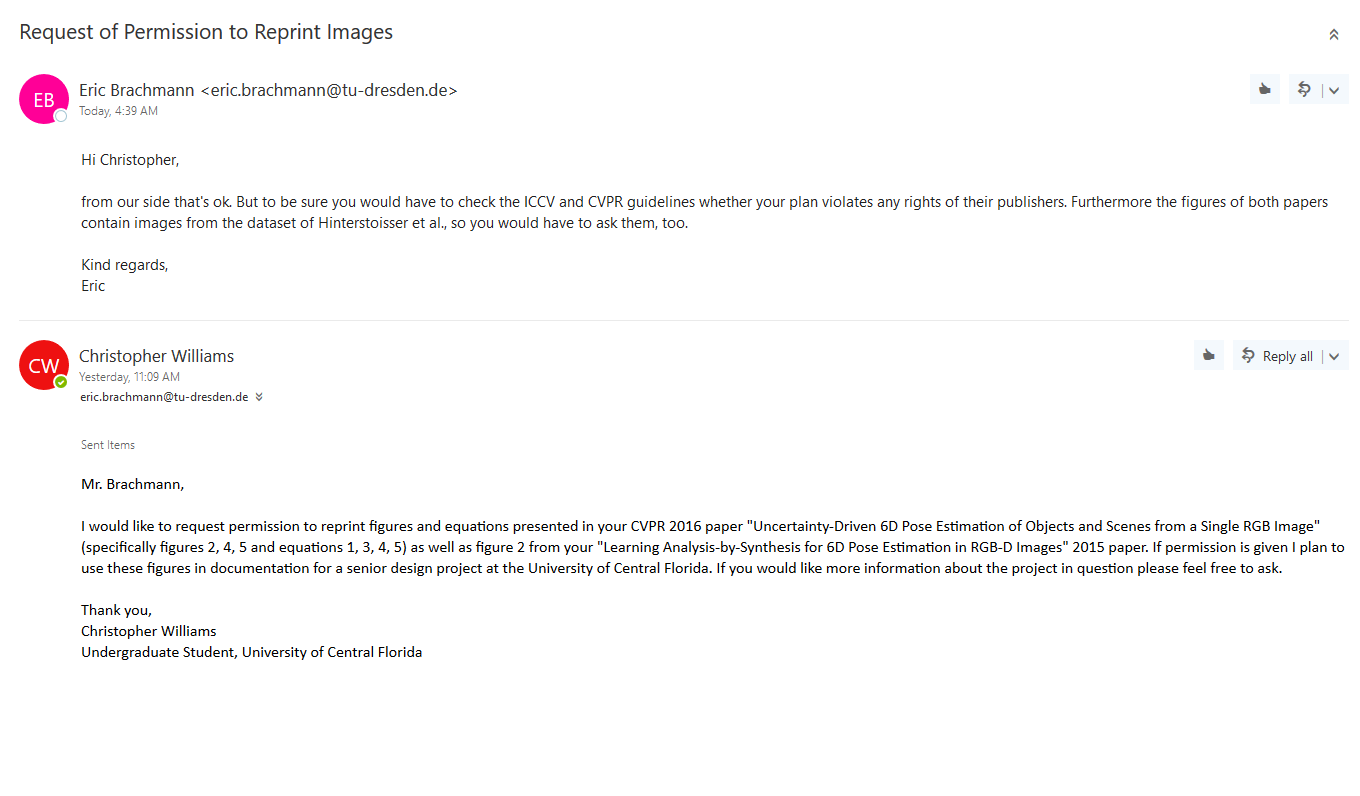
\includegraphics{Pictures/brachmannPermission.png}
\caption{Correspondence with Eric Brachmann of \autocite{bachmann}}
\end{figure}

\begin{figure}
\centering
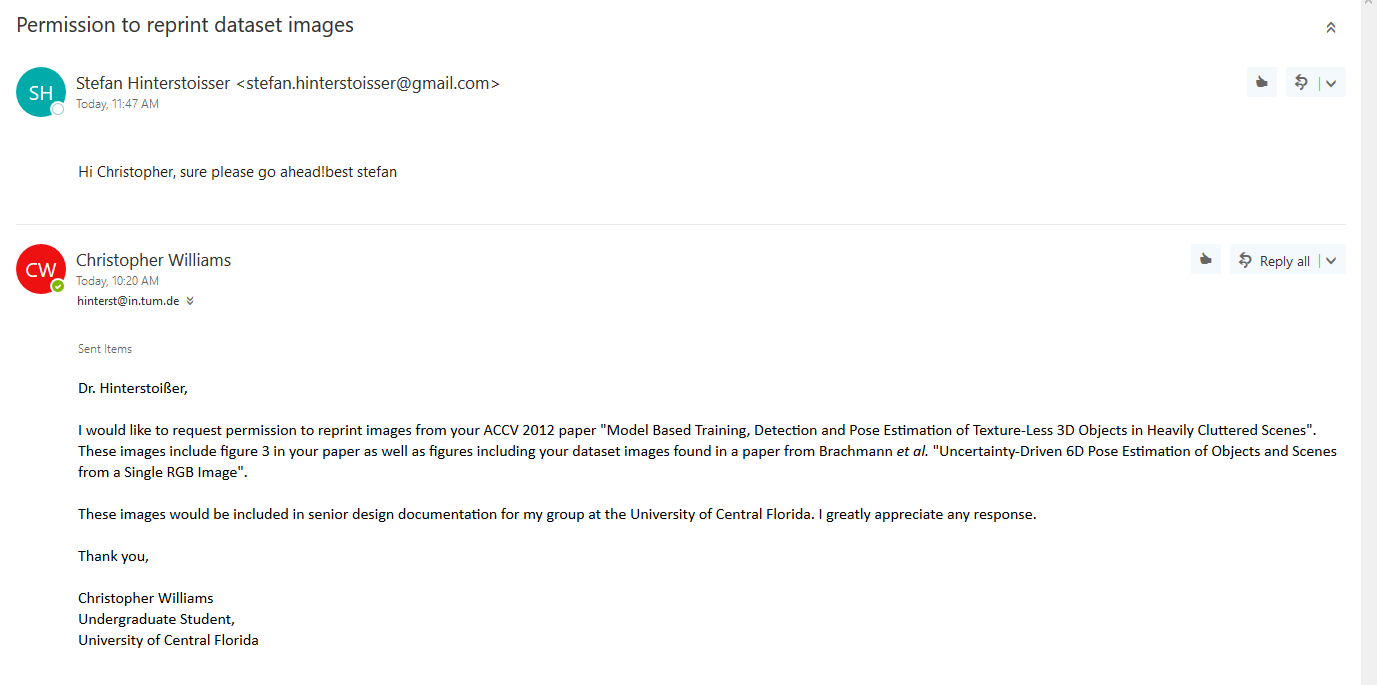
\includegraphics{Pictures/hinterstoisserPermission.png}
\caption{Correspondence with Stefan Hinterstoisser of
\autocite{hinterstoisser}}
\end{figure}

\begin{figure}
\centering
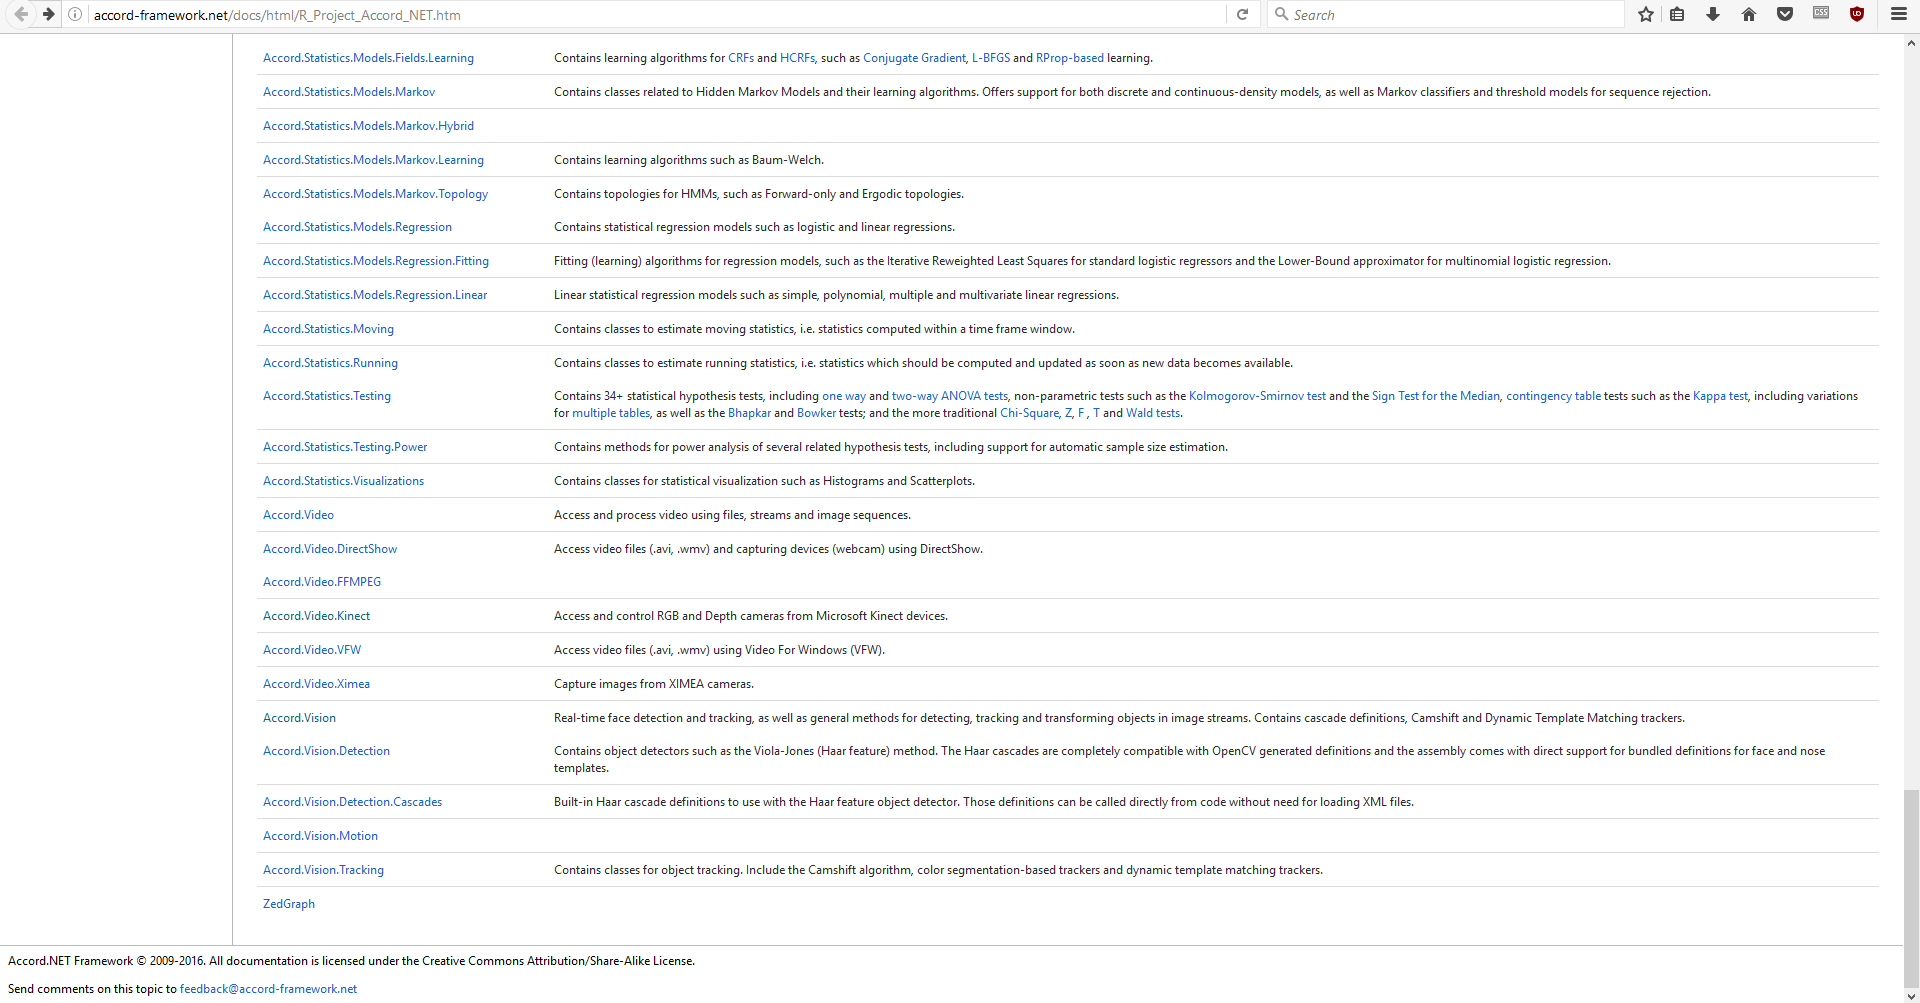
\includegraphics{Pictures/accordLicense.png}
\caption{Proof of Accord.NET License}
\end{figure}

\begin{figure}
\centering
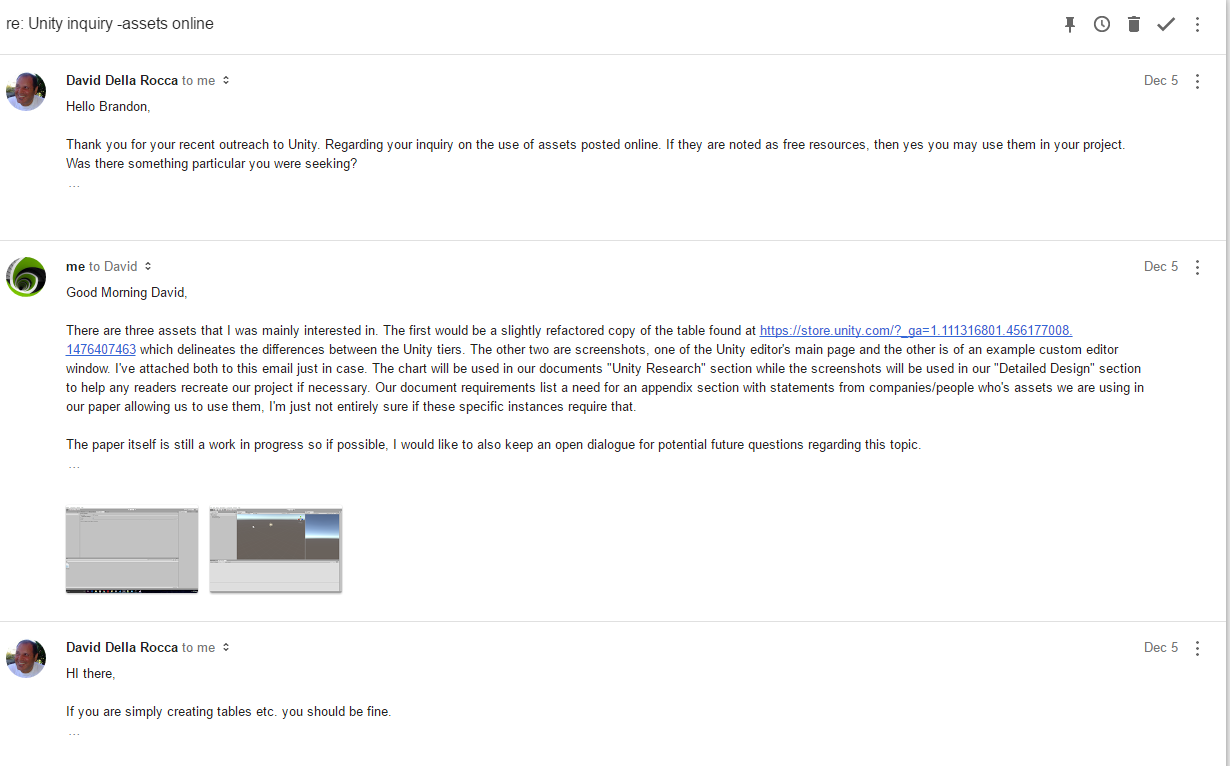
\includegraphics{Pictures/unityCorrespondence.png}
\caption{Correspondence with David Della Rocca of Unity}
\end{figure}


\includepdf[pages=-, pagecommand={}]{Appendix/AppendixB.pdf}

\printbibliography[title=References]

\end{document}